\section{Observations}
According the \ref{se:test_plan} section, this section includes the observations after performing the test plans on the \acrshort{wdias} system setup and test plan test up which is explained in the \ref{se:work_load}.

Following \ref{subse:obs_test_plan_all_60min}, \ref{subse:obs_test_plan_all_30min}, \ref{subse:obs_test_plan_all_15min} and \ref{subse:obs_test_plan_all_auto_15min} sections discussed about the observations collected with performing the Full test plan (also known as All test plan) over 60 minutes (24 data points), 30 minutes (48 data points) and 15 minutes (96 data points) by variate the request size. Then another performance test with enabling Auto Scaling as explained in \ref{subse:test_plan_metrics} for high resource utilized microservice.



\subsection{Full Test with hourly data (24 Request Size)}
\label{subse:obs_test_plan_all_60min}
After running the All test plan with 60 minutes (24 data points), it observed the data summary of \ref{tab:obs_all_60_min_summary}. It performed 311k of sample requests.
\begin{table}[]
\begin{tabulary}{\linewidth}{|L|C|C|C|C|C|C|C|C|}
\hline
Label & \# Samples & Avg & Min & Max & 90\% Line & Std. Dev. & Error \% & RPS \\ \hline
Insert Timeseries & 71826 & 28 & 13 & 2773 & 31 & 58.74 & 0.00\% & 40.5 \\ \hline
Retrieve Timeseries & 71796 & 8 & 7 & 242 & 10 & 4.18 & 0.00\% & 40.7 \\ \hline
Insert Grid & 7982 & 23 & 21 & 126 & 26 & 4.23 & 0.06\% & 4.5 \\ \hline
Retrieve Grid & 7979 & 68 & 59 & 238 & 75 & 10.11 & 0.00\% & 4.5 \\ \hline
Query: Location & 71804 & 3 & 2 & 109 & 3 & 1.52 & 0.00\% & 40.5 \\ \hline
\textbf{TOTAL} & 311182 & 127 & 0 & 2773 & 503 & 207.80 & 0.00\% & 175.4 \\ \hline
\end{tabulary}
\caption{Throughput and Latency of All test cases with 60min data}
\label{tab:obs_all_60_min_summary}
\end{table}
Insert Timeseries performed over Scalar and Vector data types with each request send with 24 data points. On average it takes 28ms to insert data into the \acrshort{wdias}, and up to 90\% percentile inserted data within 31ms. Noticeably it has 0\% of errors which means that all the request are completed successfully. On average, \acrshort{wdias} handled 40.5 \acrshort{rps} with the given workload. The performance of the Retrieve of Scalar and Vector Timeseries are similar to insert timeseries due to it depends on it.
On the other hand, Insert Grid Timeseries data perform with 23ms with almost all the request perform within same amount of time, hence the standard deviation is smaller. Retrieve Grid Timeseries data perform the same but with bit higher value of latency of 68ms. Both of insert and retrieve grid timeseries data have 4.5 \acrshort{rps} since it only get 10\% of the number of request per given time via the test plan as explain in the data ration in \ref{se:test_plan}.

\begin{figure}[htp]
    \centering
    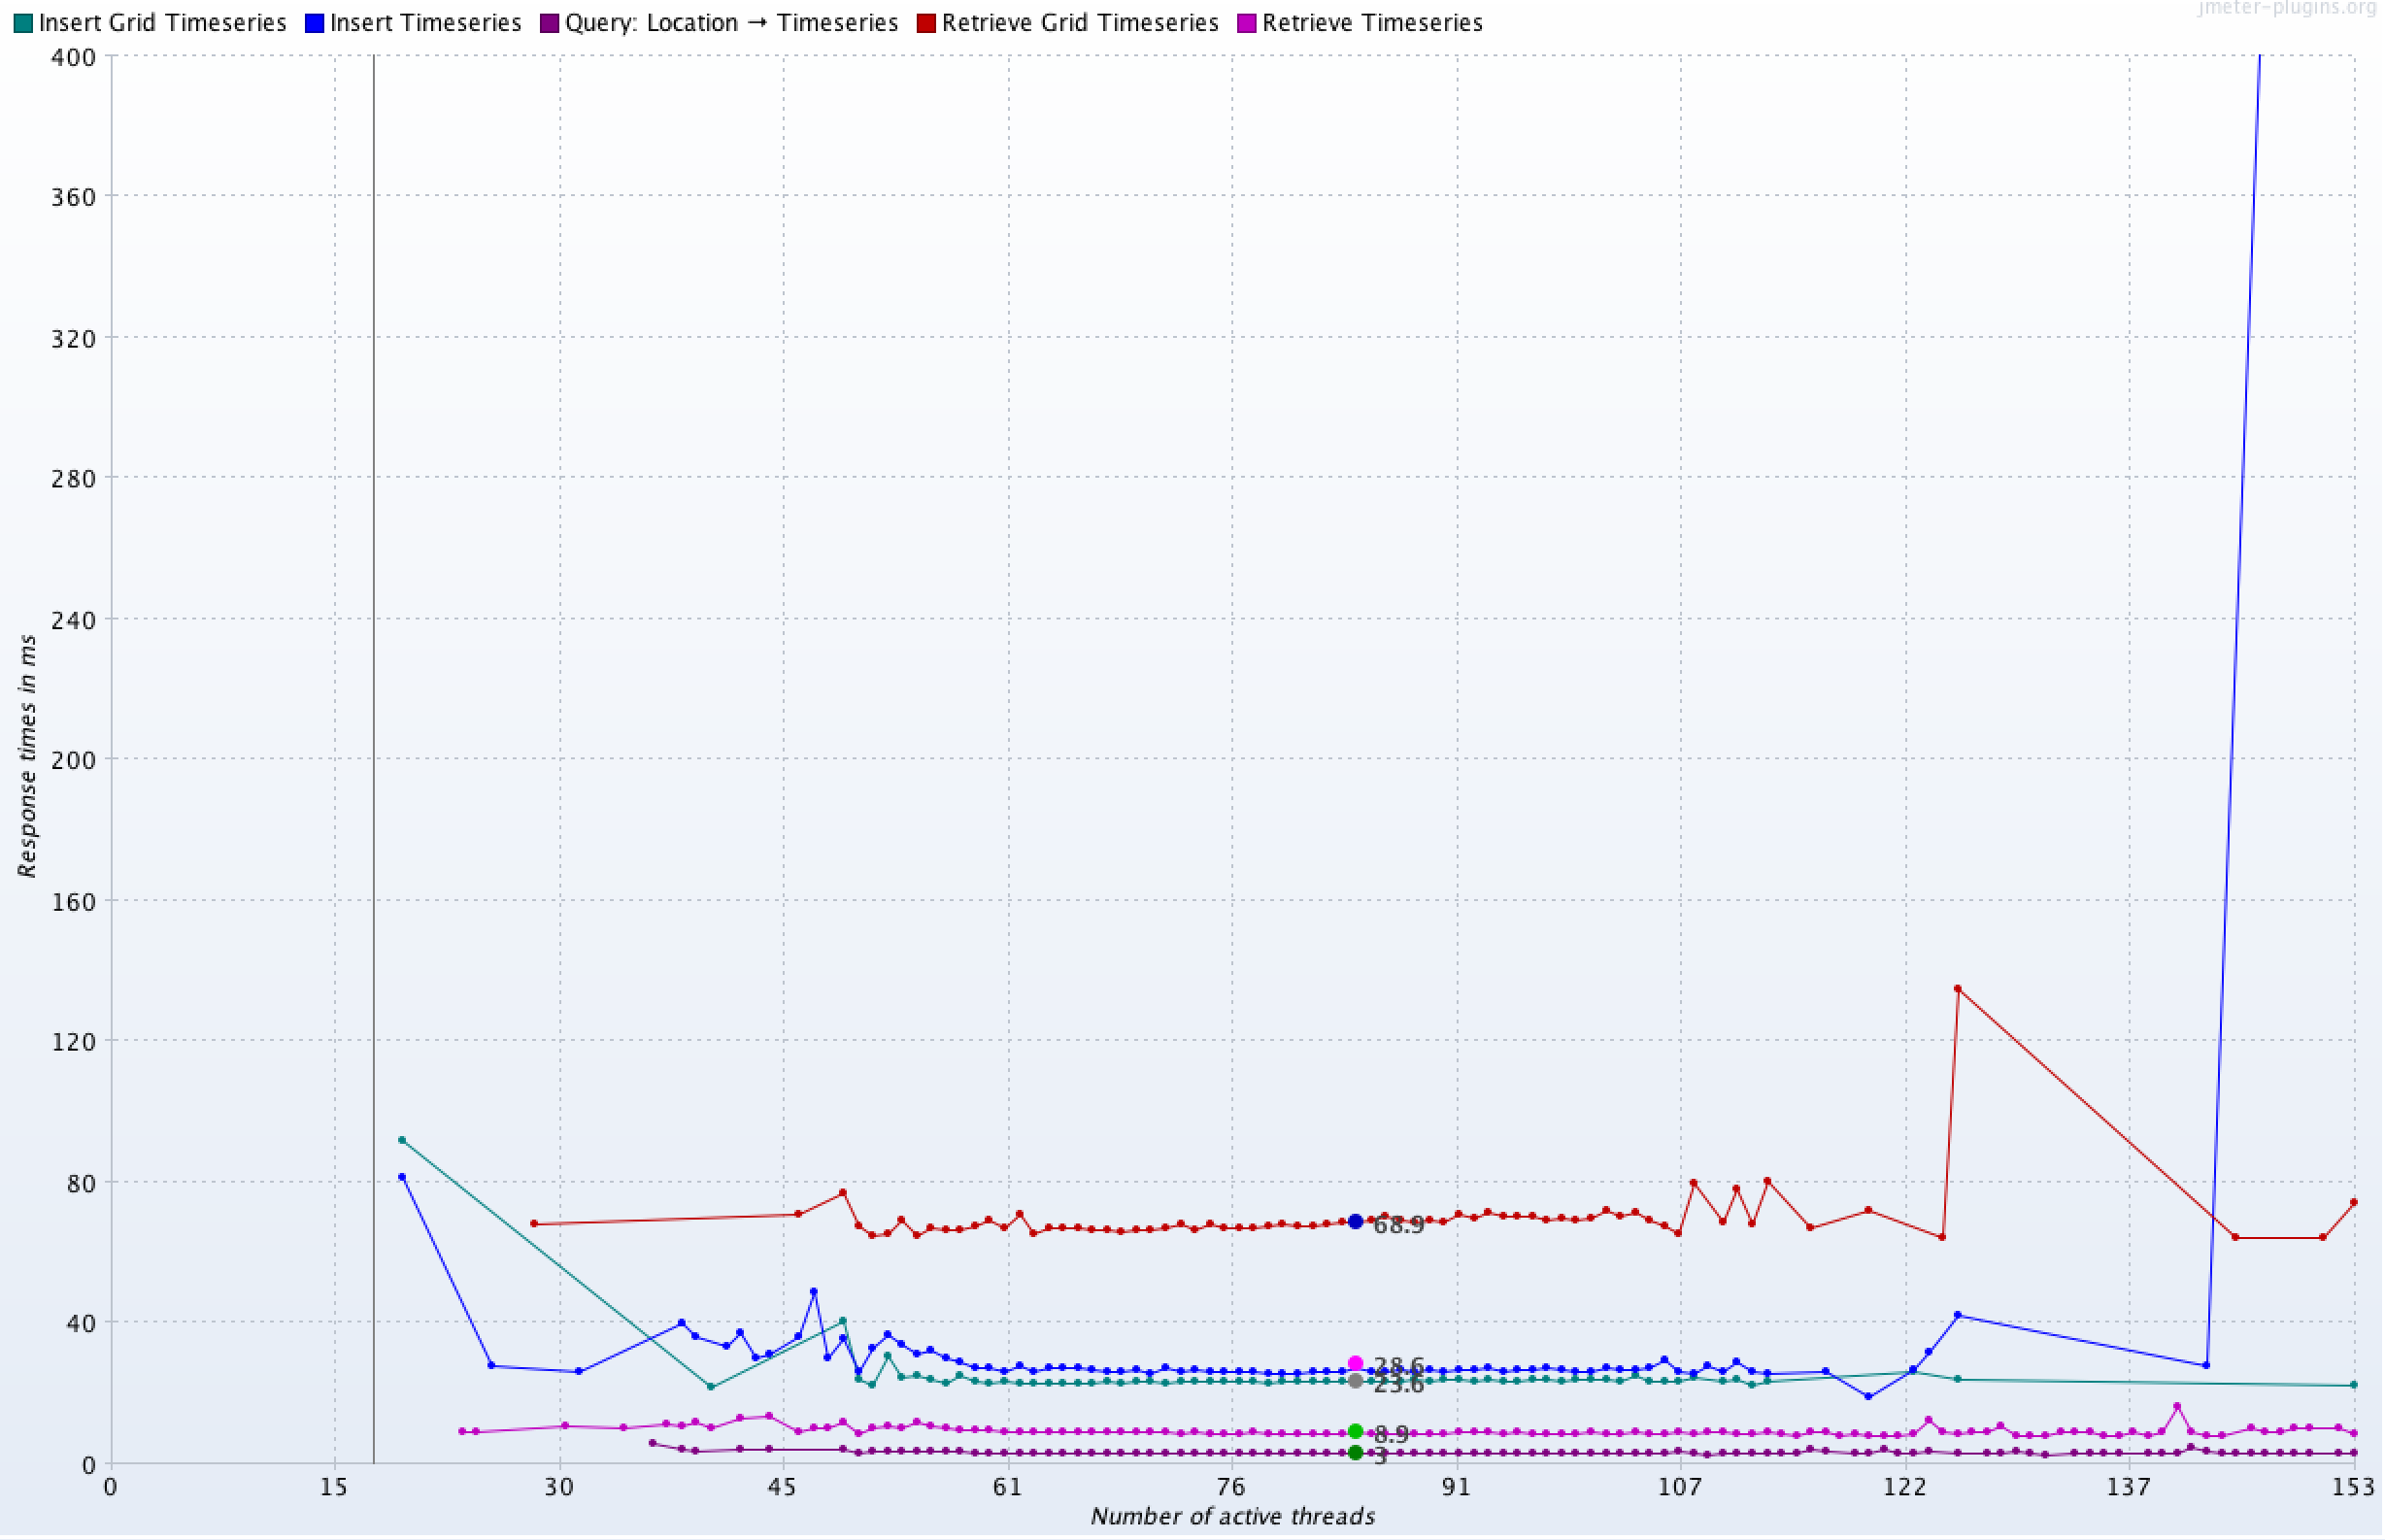
\includegraphics[width=0.8\textwidth]{results/obs/all/obs_all_60m_response_times_vs_threads.png}
    \caption{Performance All Test 60 minutes - Response Time vs Threads}
    \label{fi:test_obs_all_60m_response_vs_threads}
\end{figure}
\ref{fi:test_obs_all_60m_response_vs_threads} show the response time against the number of active threads. As the graph show, the response time kept same while increasing the number of active threads against each test case. This shows the scalability of the \acrshort{wdias}, since the system able to process more requests without a significant change in the latency.
When number of active threads increased more than 122, the \ref{fi:test_obs_all_60m_response_vs_threads} show uncertainty in the inserting and retrieving Scalar and Vector data.

\begin{figure}[htp]
    \centering
    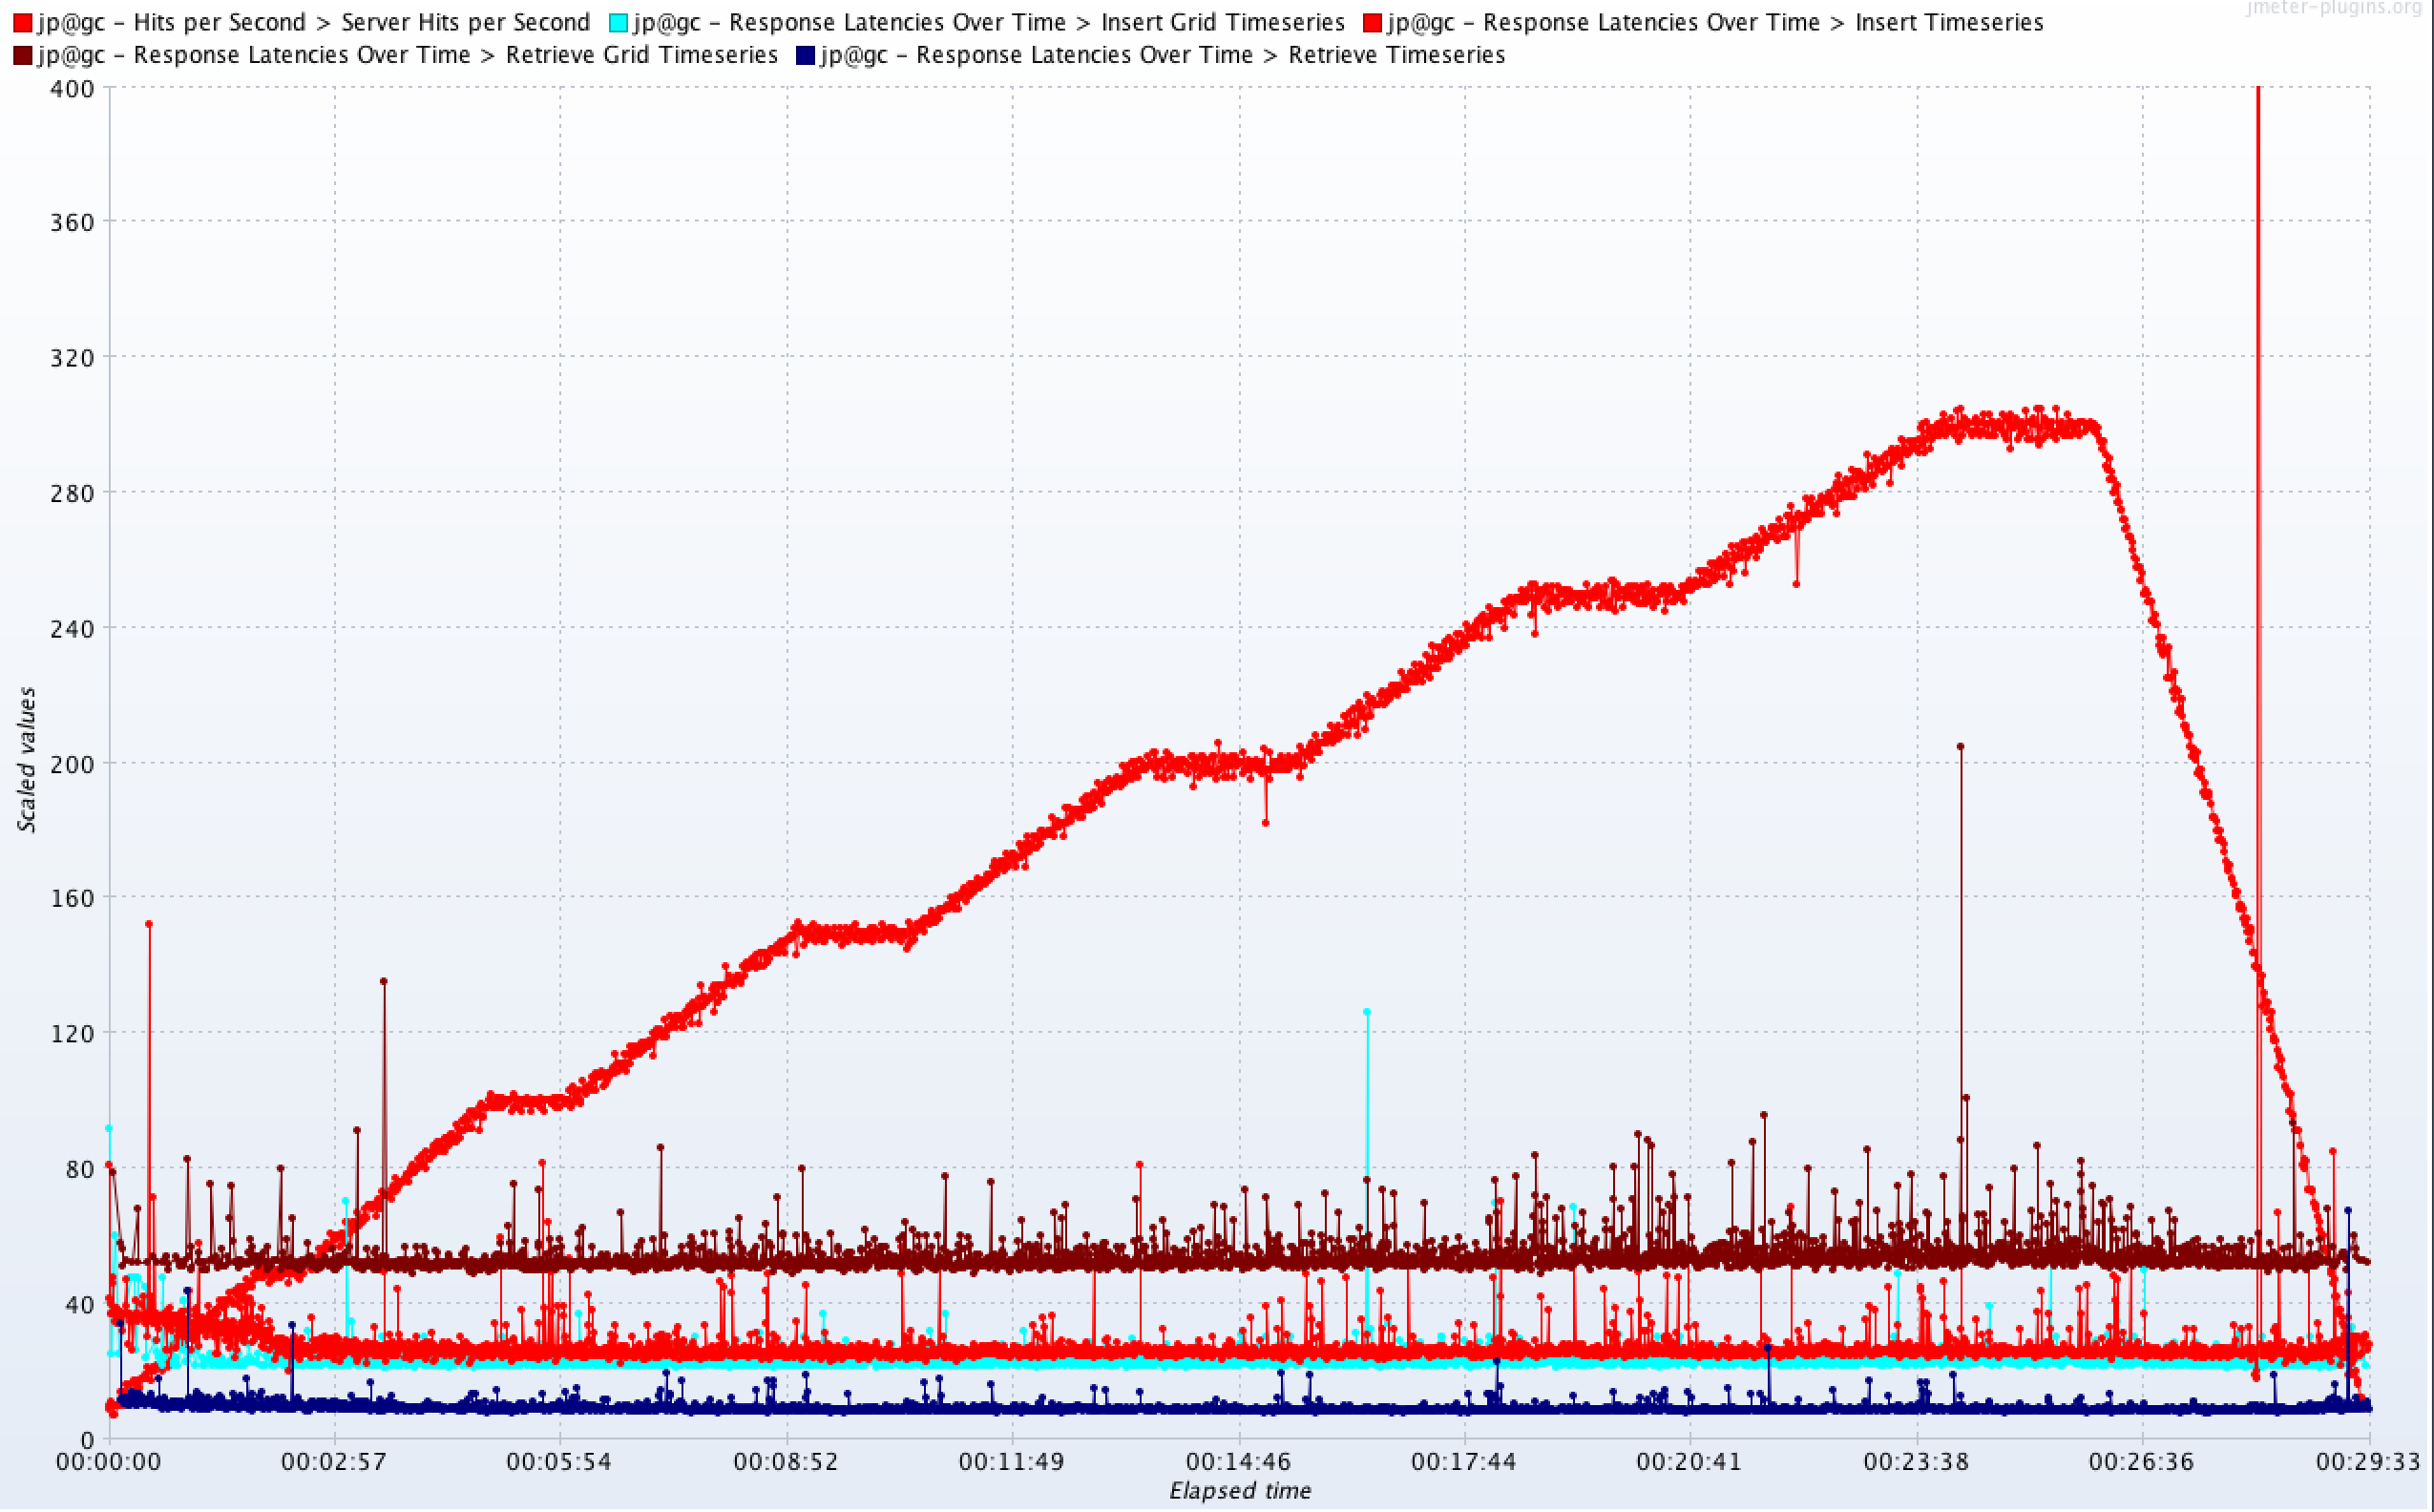
\includegraphics[width=0.8\textwidth]{results/obs/all/obs_all_60m_res_latencies_against_hits.png}
    \caption{Performance All Test 60 minutes - Latency against server hits}
    \label{fi:test_obs_all_60m_latency}
\end{figure}
\ref{fi:test_obs_all_60m_latency} graph provides a better overview of the variation of latency over elapsed time of the test plan against number of server hits per second.
The conclusion of giving static latency while increasing the number of requests in \ref{fi:test_obs_all_60m_response_vs_threads} can further prove with this graph, since \ref{fi:test_obs_all_60m_latency} graph gives in details overview over the test plan time span.



\subsection{Full Test with 30min data (48 Request Size)}
\label{subse:obs_test_plan_all_30min}
This section \ref{subse:obs_test_plan_all_30min} discussed about the All test plan performance with 30 minutes data which means 48 data points per each request in Scalar and Vector timeseries, and 48 ASCII Grid files per each insert request. It performed round up to 311k of sample requests which is almost similar to \ref{subse:obs_test_plan_all_60min} processed samples.
\begin{table}[]
\begin{tabulary}{\linewidth}{|L|C|C|C|C|C|C|C|C|}
\hline
Label & \# Samples & Average & Min & Max & 90\% Line & Std. Dev. & Error \% & RPS \\ \hline
Insert Timeseries & 71759 & 29 & 14 & 1699 & 32 & 50.97 & 0.00\% & 40.5 \\ \hline
Retrieve Timeseries & 71730 & 9 & 7 & 1033 & 10 & 6.04 & 0.00\% & 40.6 \\ \hline
Insert Grid & 7972 & 44 & 40 & 162 & 49 & 8.17 & 0.08\% & 4.5 \\ \hline
Retrieve Grid & 7971 & 81 & 67 & 284 & 93 & 15.15 & 0.00\% & 4.5 \\ \hline
Query: Location & 71734 & 3 & 2 & 110 & 3 & 1.90 & 0.00\% & 40.5 \\ \hline
TOTAL & 310878 & 129 & 0 & 1699 & 503 & 207.10 & 0.00\% & 175.3 \\ \hline
\end{tabulary}
\caption{Throughput and Latency of All test cases with 30min data}
\label{tab:obs_all_30_min_summary}
\end{table}
\ref{tab:obs_all_30_min_summary} shows the response latency summary details and \acrshort{rps} as explained in \ref{subse:obs_test_plan_all_60min}. And the results are almost similar to the observations in \ref{tab:obs_all_60_min_summary}. This implies that, even the request size is increased, the \acrshort{wdias} can perform better same as the with smaller size of data.

\begin{figure}[htp]
    \centering
    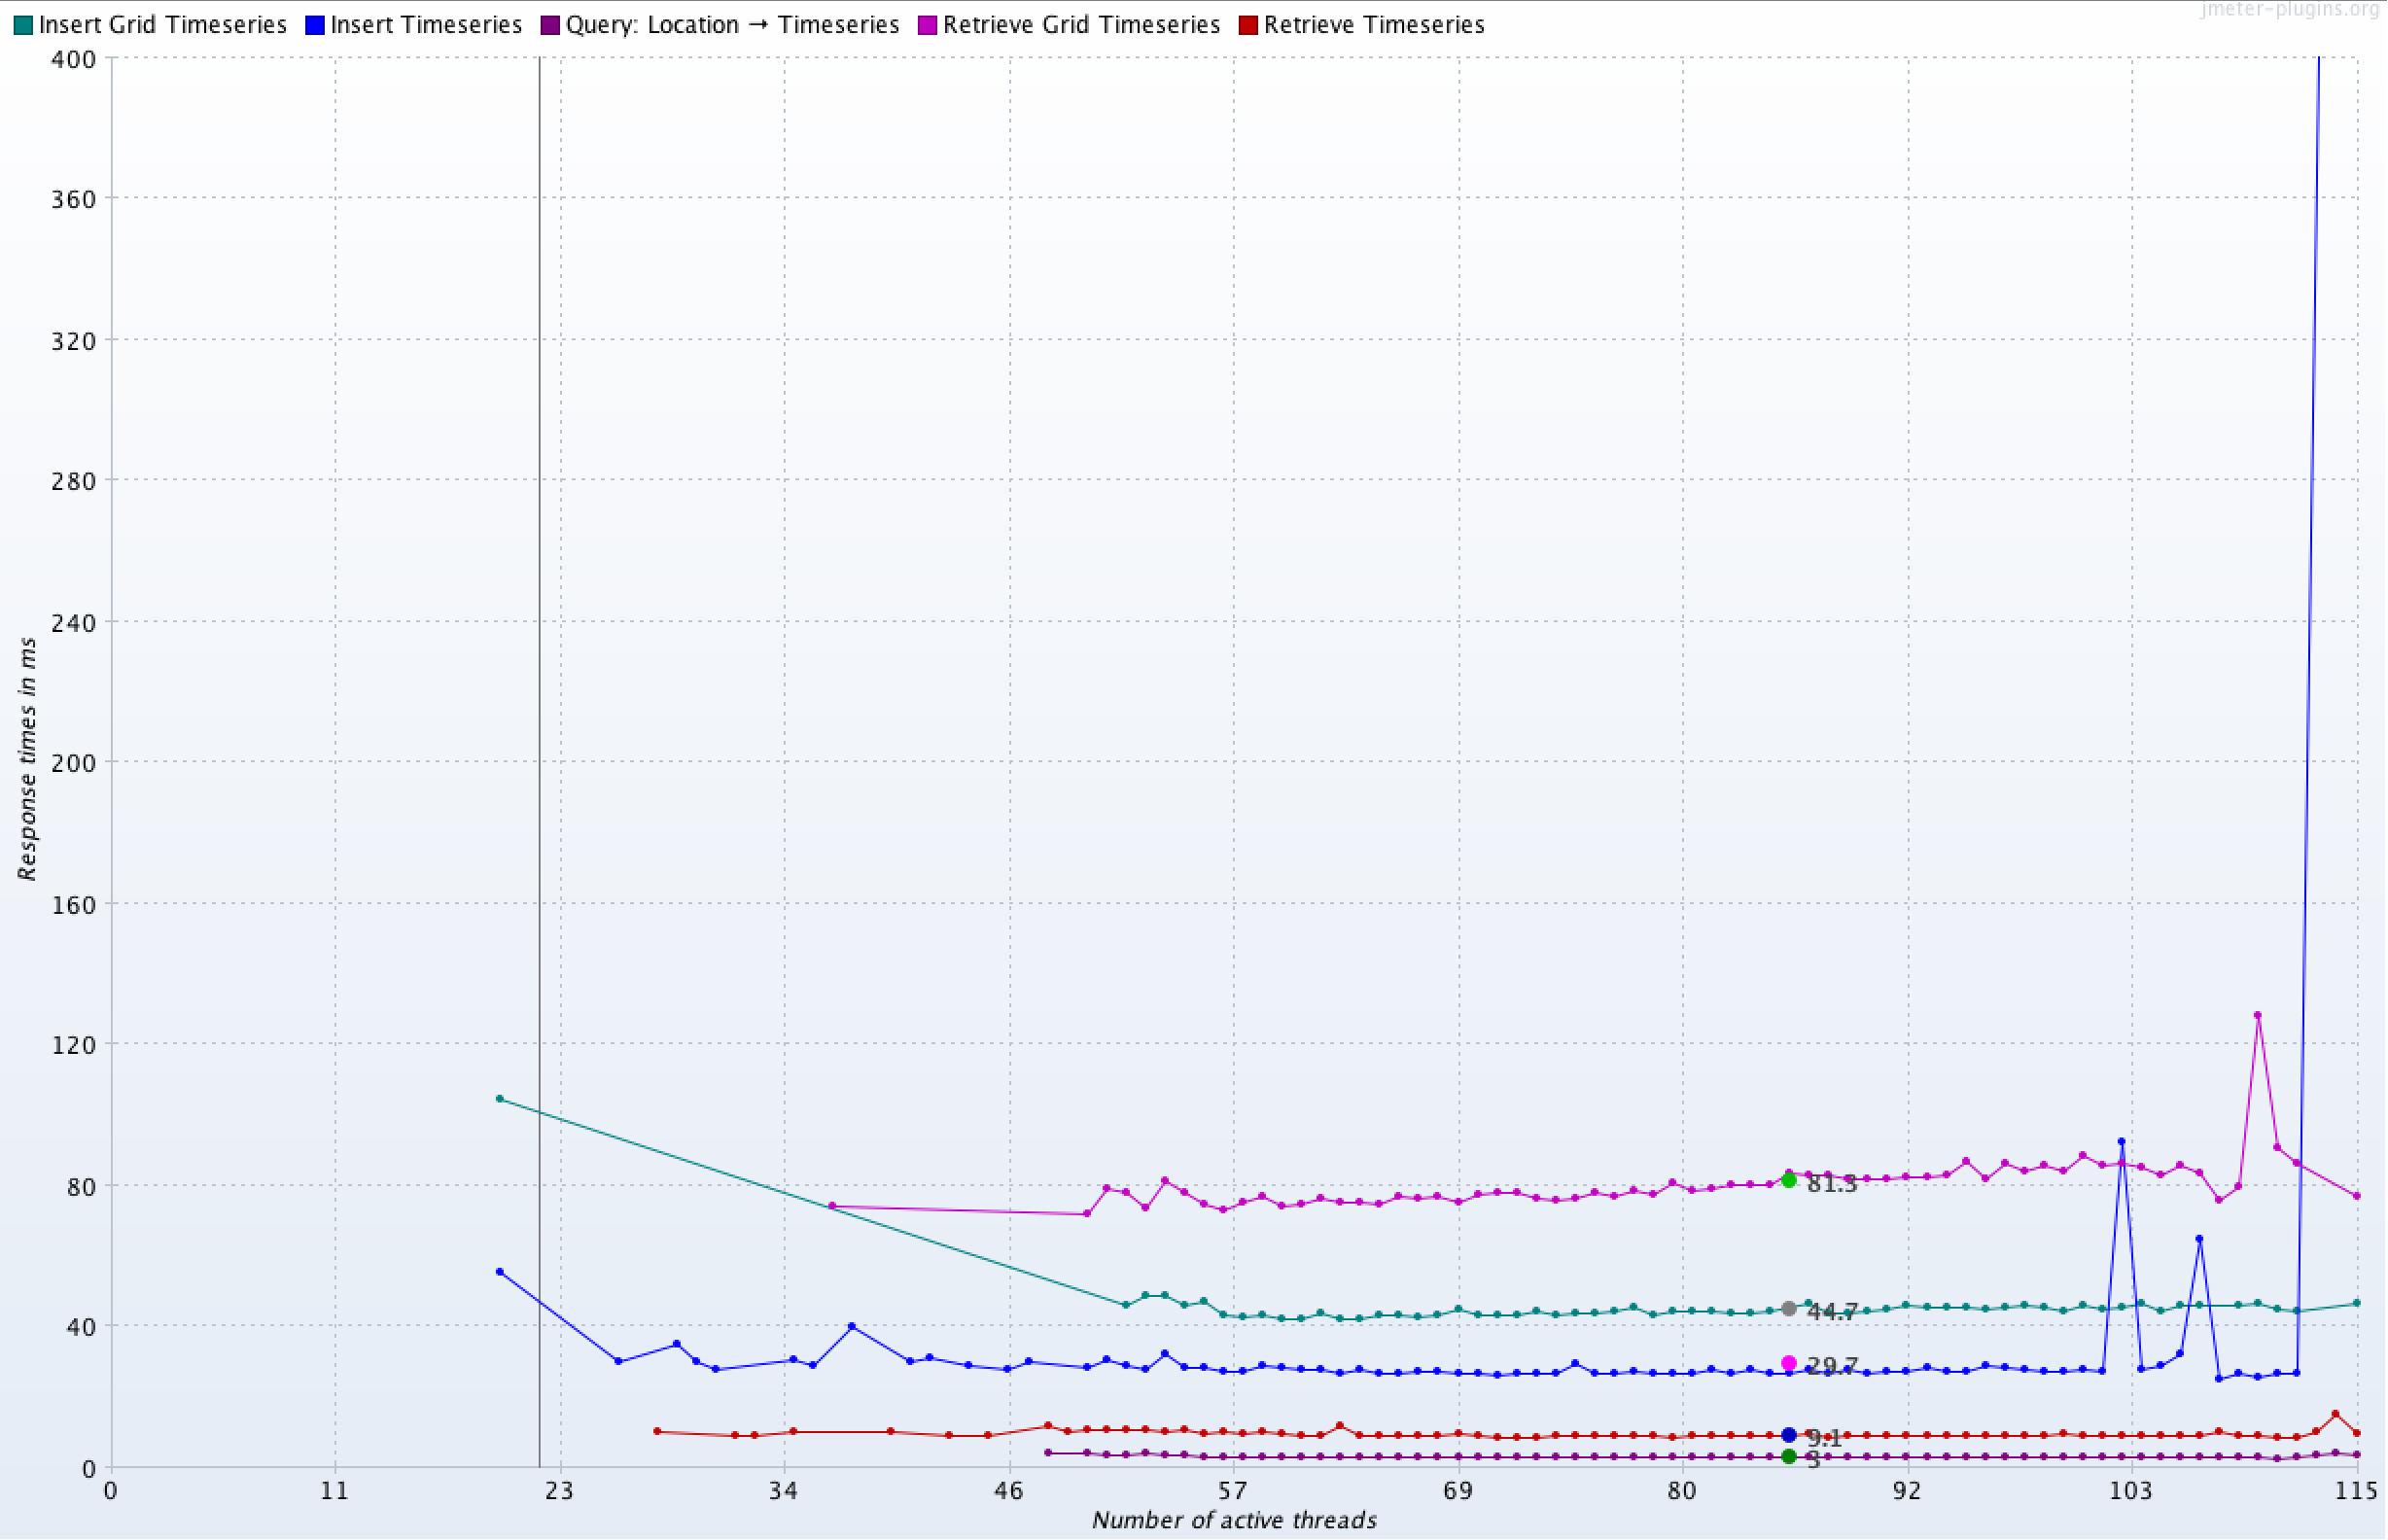
\includegraphics[width=0.8\textwidth]{results/obs/all/obs_all_30m_response_times_vs_threads.png}
    \caption{Performance All Test 30 minutes - Response Time vs Threads}
    \label{fi:test_obs_all_30m_response_vs_threads}
\end{figure}
\ref{fi:test_obs_all_30m_response_vs_threads} show the response time against the number of active threads for 30min data. As the graph show, the response time kept same while increasing the number of active threads against each test case. This shows the scalability of the \acrshort{wdias}, since the system able to process more requests without a significant change in the latency.
When number of active threads increased more than 110, the \ref{fi:test_obs_all_30m_response_vs_threads} show uncertainty in the inserting and retrieving Scalar and Vector data. This graph is similar to the \ref{fi:test_obs_all_60m_response_vs_threads}, but the active thread count goes down as a result of increasing the request size.

\begin{figure}[htp]
    \centering
    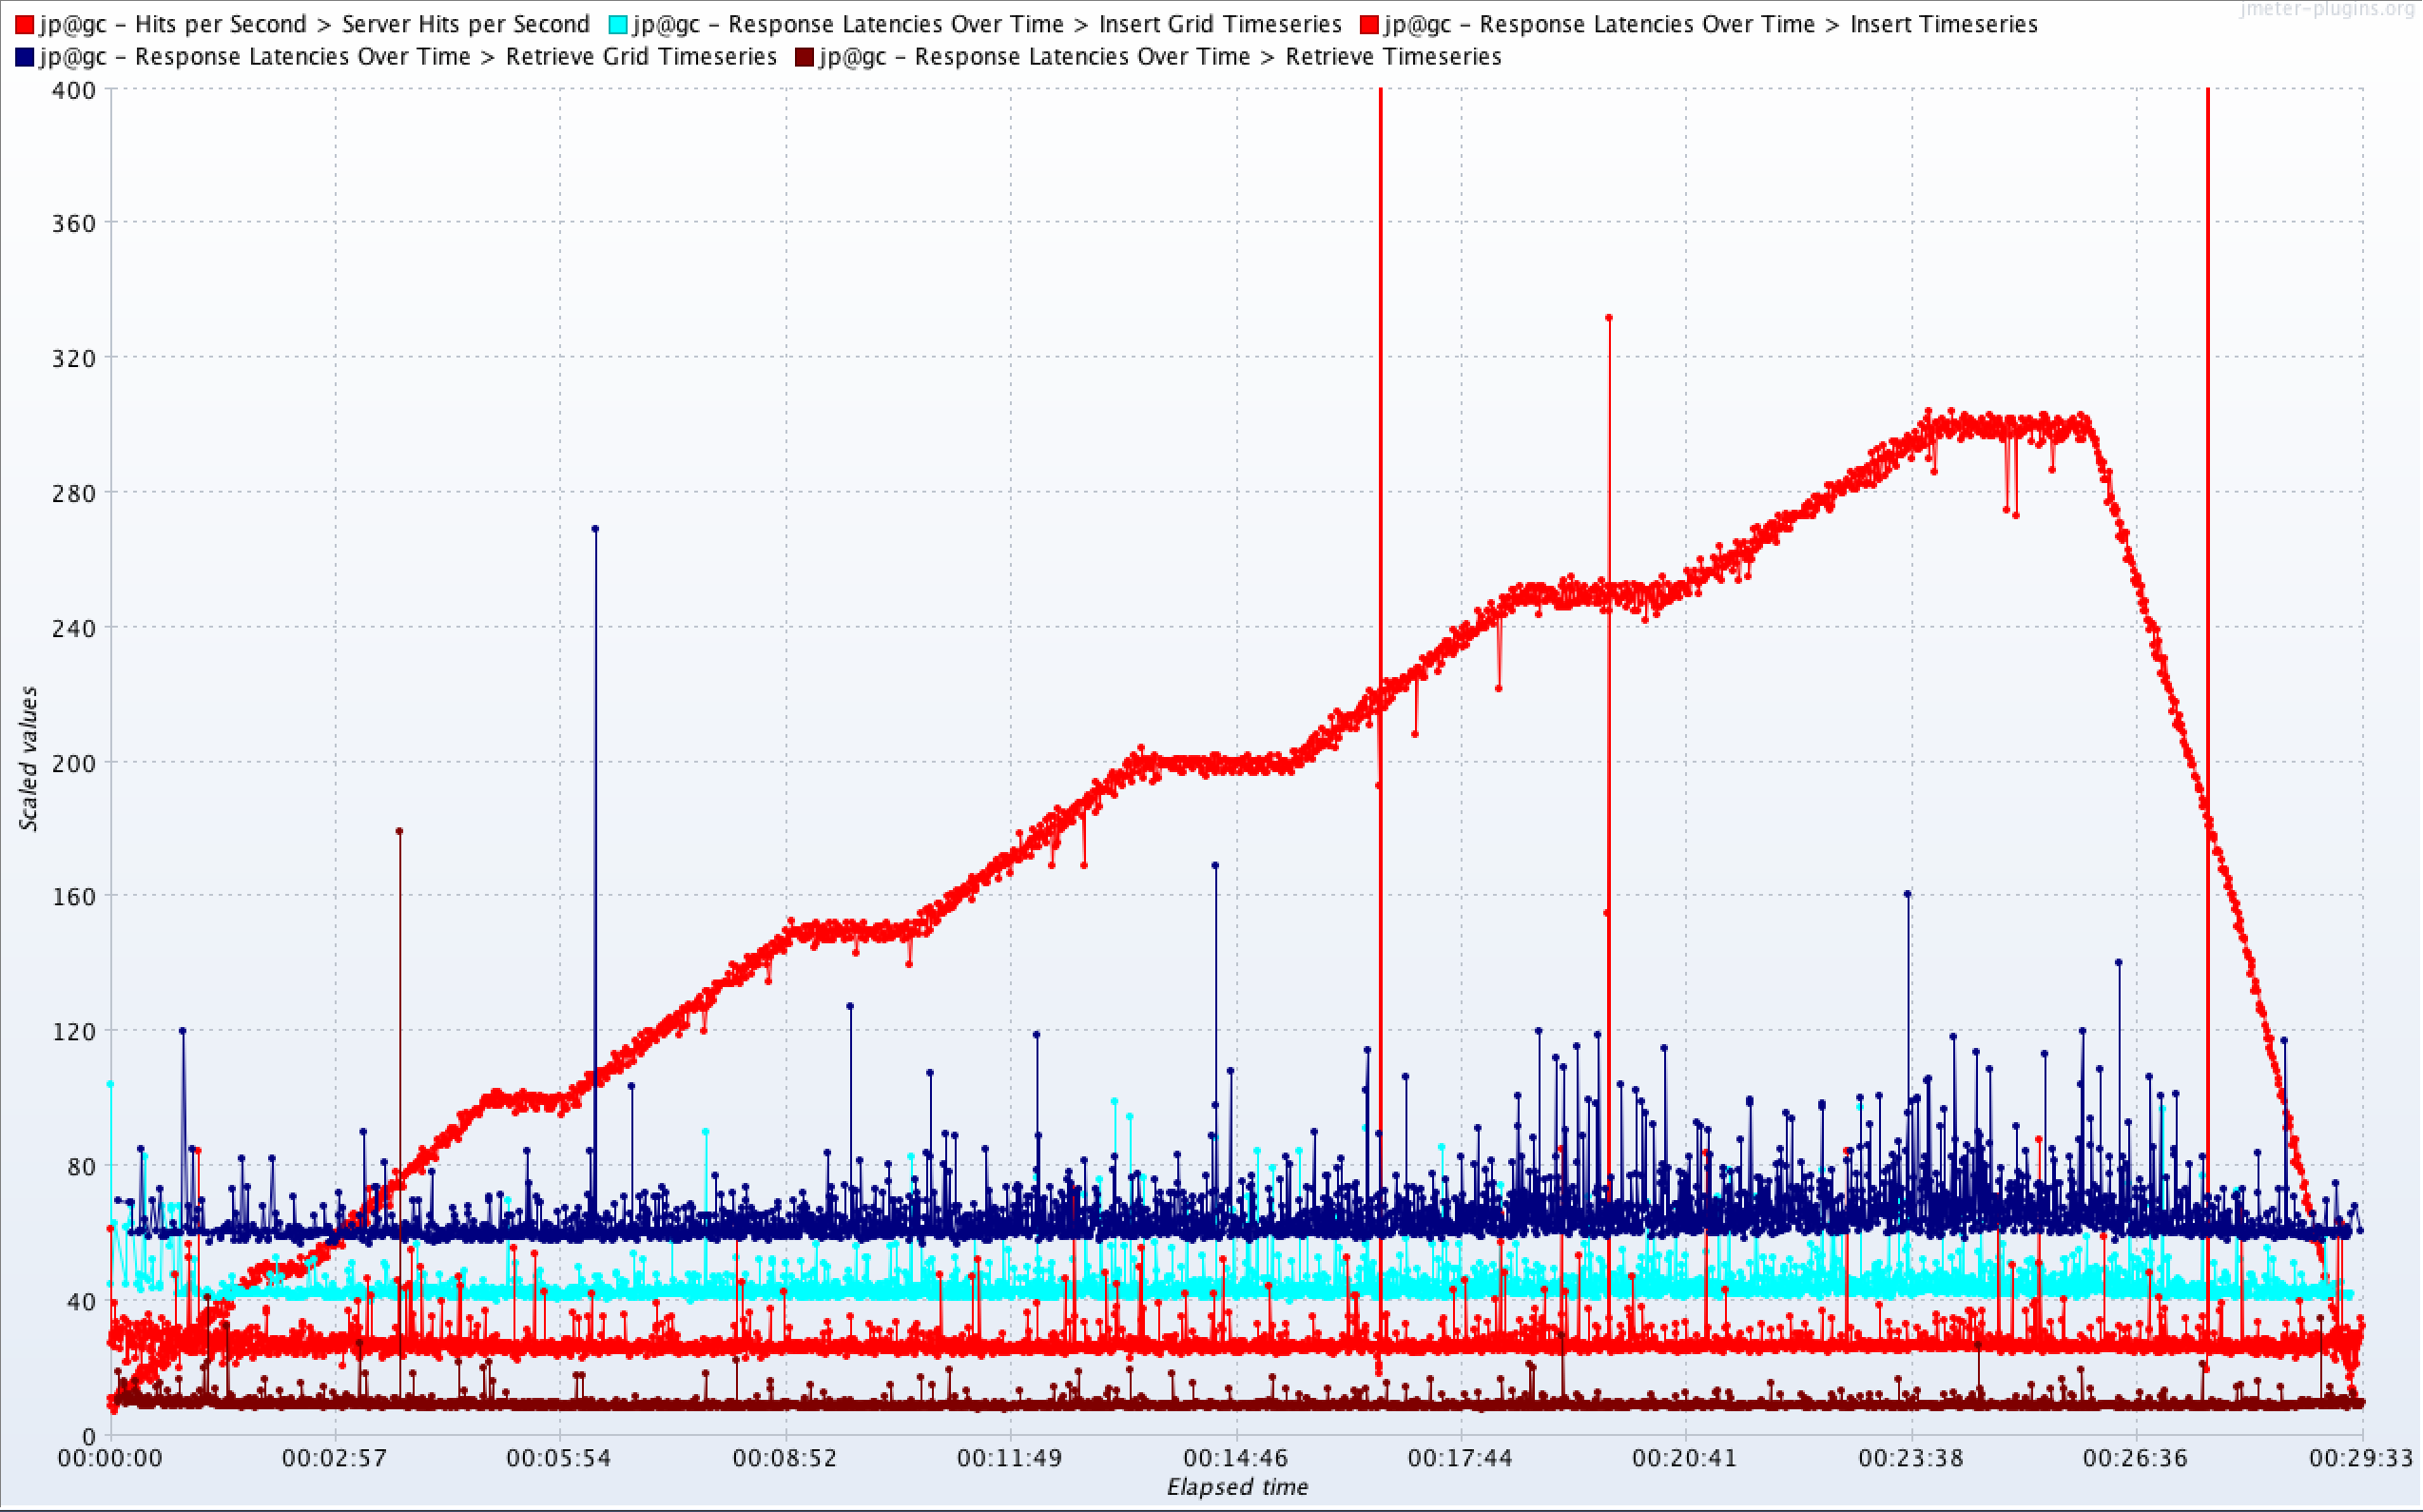
\includegraphics[width=0.8\textwidth]{results/obs/all/obs_all_30m_res_latencies_against_hits.png}
    \caption{Performance All Test 30 minutes - Latency against server hits}
    \label{fi:test_obs_all_30m_latency}
\end{figure}
\ref{fi:test_obs_all_30m_latency} graph provides a better overview of the variation of latency over elapsed time of the test plan against number of server hits per second.
This graph also conclude that, over the time latency does not change very much. But during the peak load, it shows some variation in insert and retrieve of Grid timeseries.
When compared to \ref{fi:test_obs_all_60m_latency}, the latency for insert and retrieve Grid timeseries increase by some amount.



\subsection{Full Test with 15min data (96 Request Size)}
\label{subse:obs_test_plan_all_15min}
This section \ref{subse:obs_test_plan_all_15min} discussed about the All test plan performance with 15 minutes data which means 96 data points per each request in Scalar and Vector timeseries, and 48 ASCII Grid files per each insert Grid timeseries request. These requests are four times larger than the \ref{subse:obs_test_plan_all_60min} request size. It performed approximately 311k of sample requests which is almost similar to \ref{subse:obs_test_plan_all_30min} processed samples.
\begin{table}[]
\begin{tabulary}{\linewidth}{|L|C|C|C|C|C|C|C|C|}
\hline
Label & \# Samples & Average & Min & Max & 90\% Line & Std. Dev. & Error \% & RPS \\ \hline
Insert Timeseries & 71775 & 30 & 12 & 1719 & 41 & 51.71 & 0.00\% & 40.5 \\ \hline
Retrieve Timeseries & 71736 & 23 & 8 & 1623 & 32 & 50.18 & 0.00\% & 40.6 \\ \hline
Insert Grid & 7975 & 91 & 77 & 279 & 112 & 19.58 & 1.42\% & 4.5 \\ \hline
Retrieve Grid & 7972 & 118 & 80 & 876 & 165 & 56.15 & 0.00\% & 4.5 \\ \hline
Query: Location & 71749 & 3 & 2 & 130 & 4 & 2.32 & 0.00\% & 40.5 \\ \hline
\textbf{TOTAL} & 310934 & 134 & 0 & 1719 & 503 & 206.40 & 0.04\% & 175.4 \\ \hline
\end{tabulary}
\caption{Throughput and Latency of All test cases with 15min data}
\label{tab:obs_all_15_min_summary}
\end{table}
\ref{tab:obs_all_15_min_summary} shows the response latency summary details and \acrshort{rps} as same as explained in \ref{subse:obs_test_plan_all_30min}. And the latency observations are increased by some amount when compared to the observations in \ref{tab:obs_all_30_min_summary}. Noticeably retrieving latency of all type of data types increased by considerable amount. Same following the trend, standard deviation of retrieve timeseries data increased my considerable amount for all the types. We can assume that more writing to the databases affected on reads as well. Event the request data size increased by 4x time, the \acrshort{wdias} were able to handle them without any significant performance issues. And the system able to provide the same throughput as \ref{tab:obs_all_30_min_summary}.

\begin{figure}[htp]
    \centering
    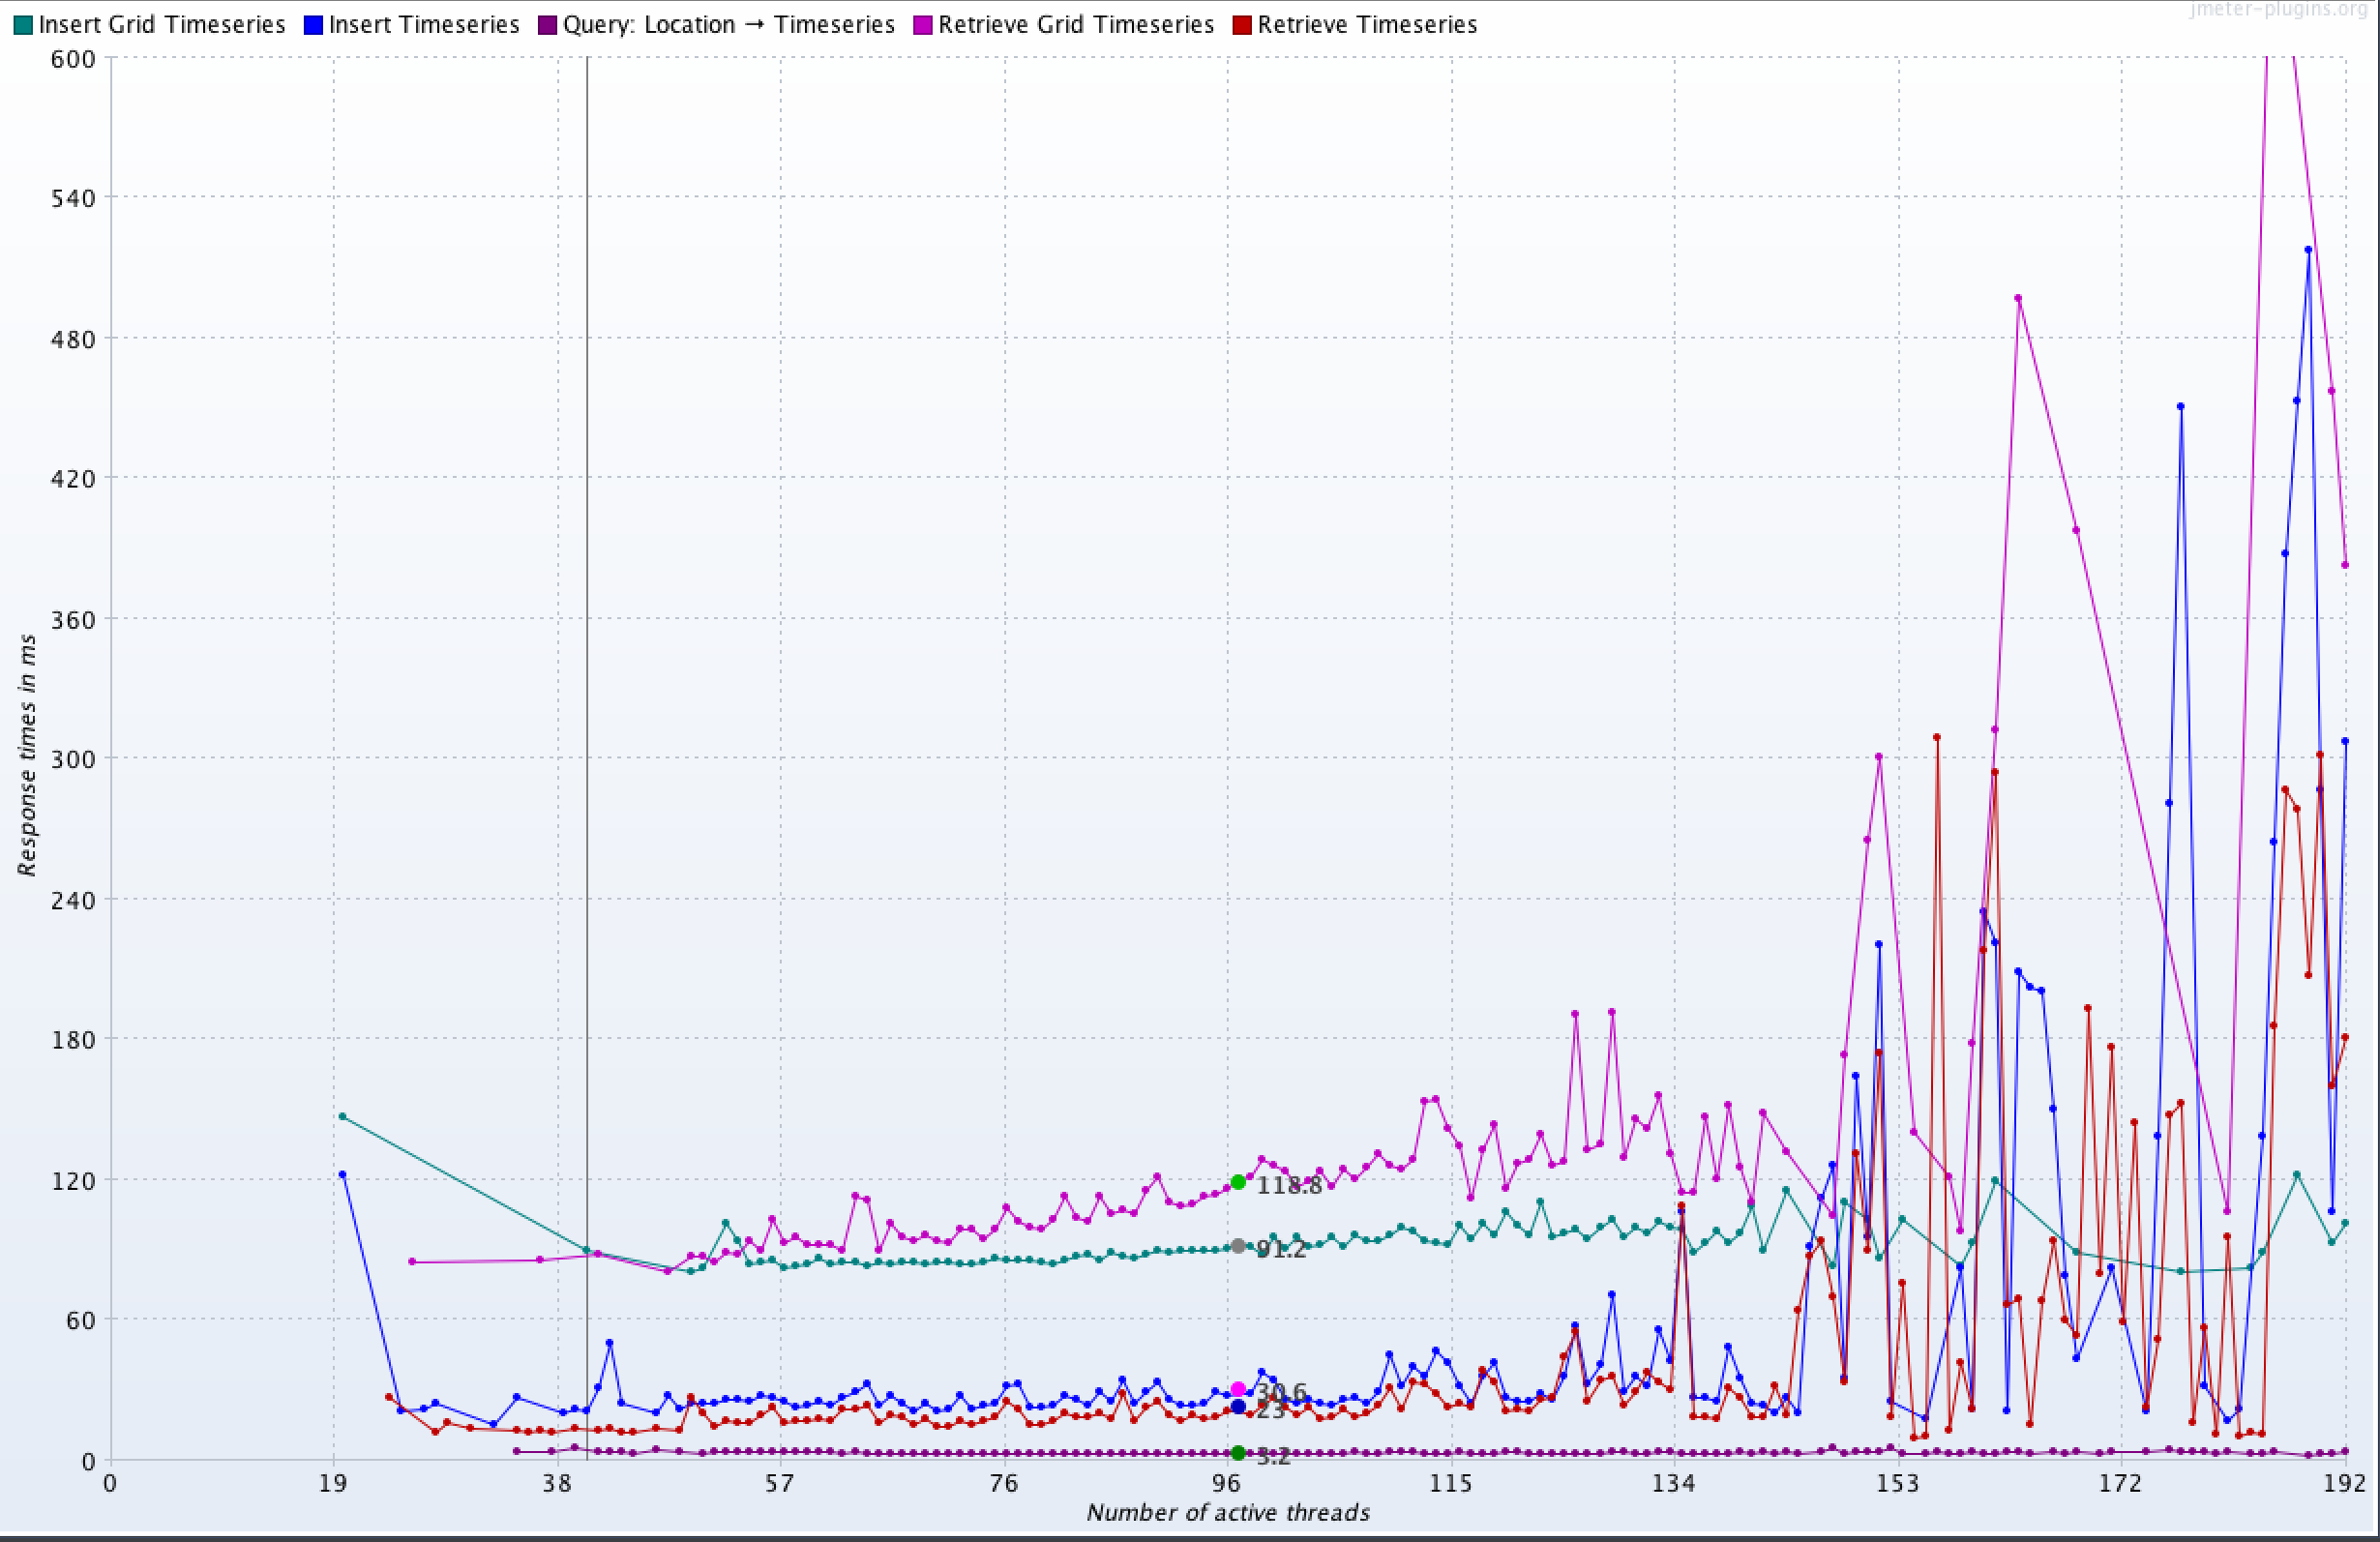
\includegraphics[width=0.8\textwidth]{results/obs/all/obs_all_15m_response_times_vs_threads.png}
    \caption{Performance Test - Response Time vs Active Threads}
    \label{fi:test_obs_all_15m_response_vs_threads}
\end{figure}
\ref{fi:test_obs_all_15m_response_vs_threads} show the response time against the number of active threads for 15min data. As the graph show, the response time kept same while increasing the number of active threads against each test case. When number of active threads increased more than 140, the \ref{fi:test_obs_all_15m_response_vs_threads} show uncertainty in the inserting and retrieving all data types. The latency of insert and retrieve Grid timeseries data goes up compared to \ref{fi:test_obs_all_30m_response_vs_threads}.
With higher request size, it become to notice the latency also increase by a small factor when the number of active thread increased. This can clearly notice on with insert and retrieval of Grid timeseries data.

\begin{figure}[htp]
    \centering
    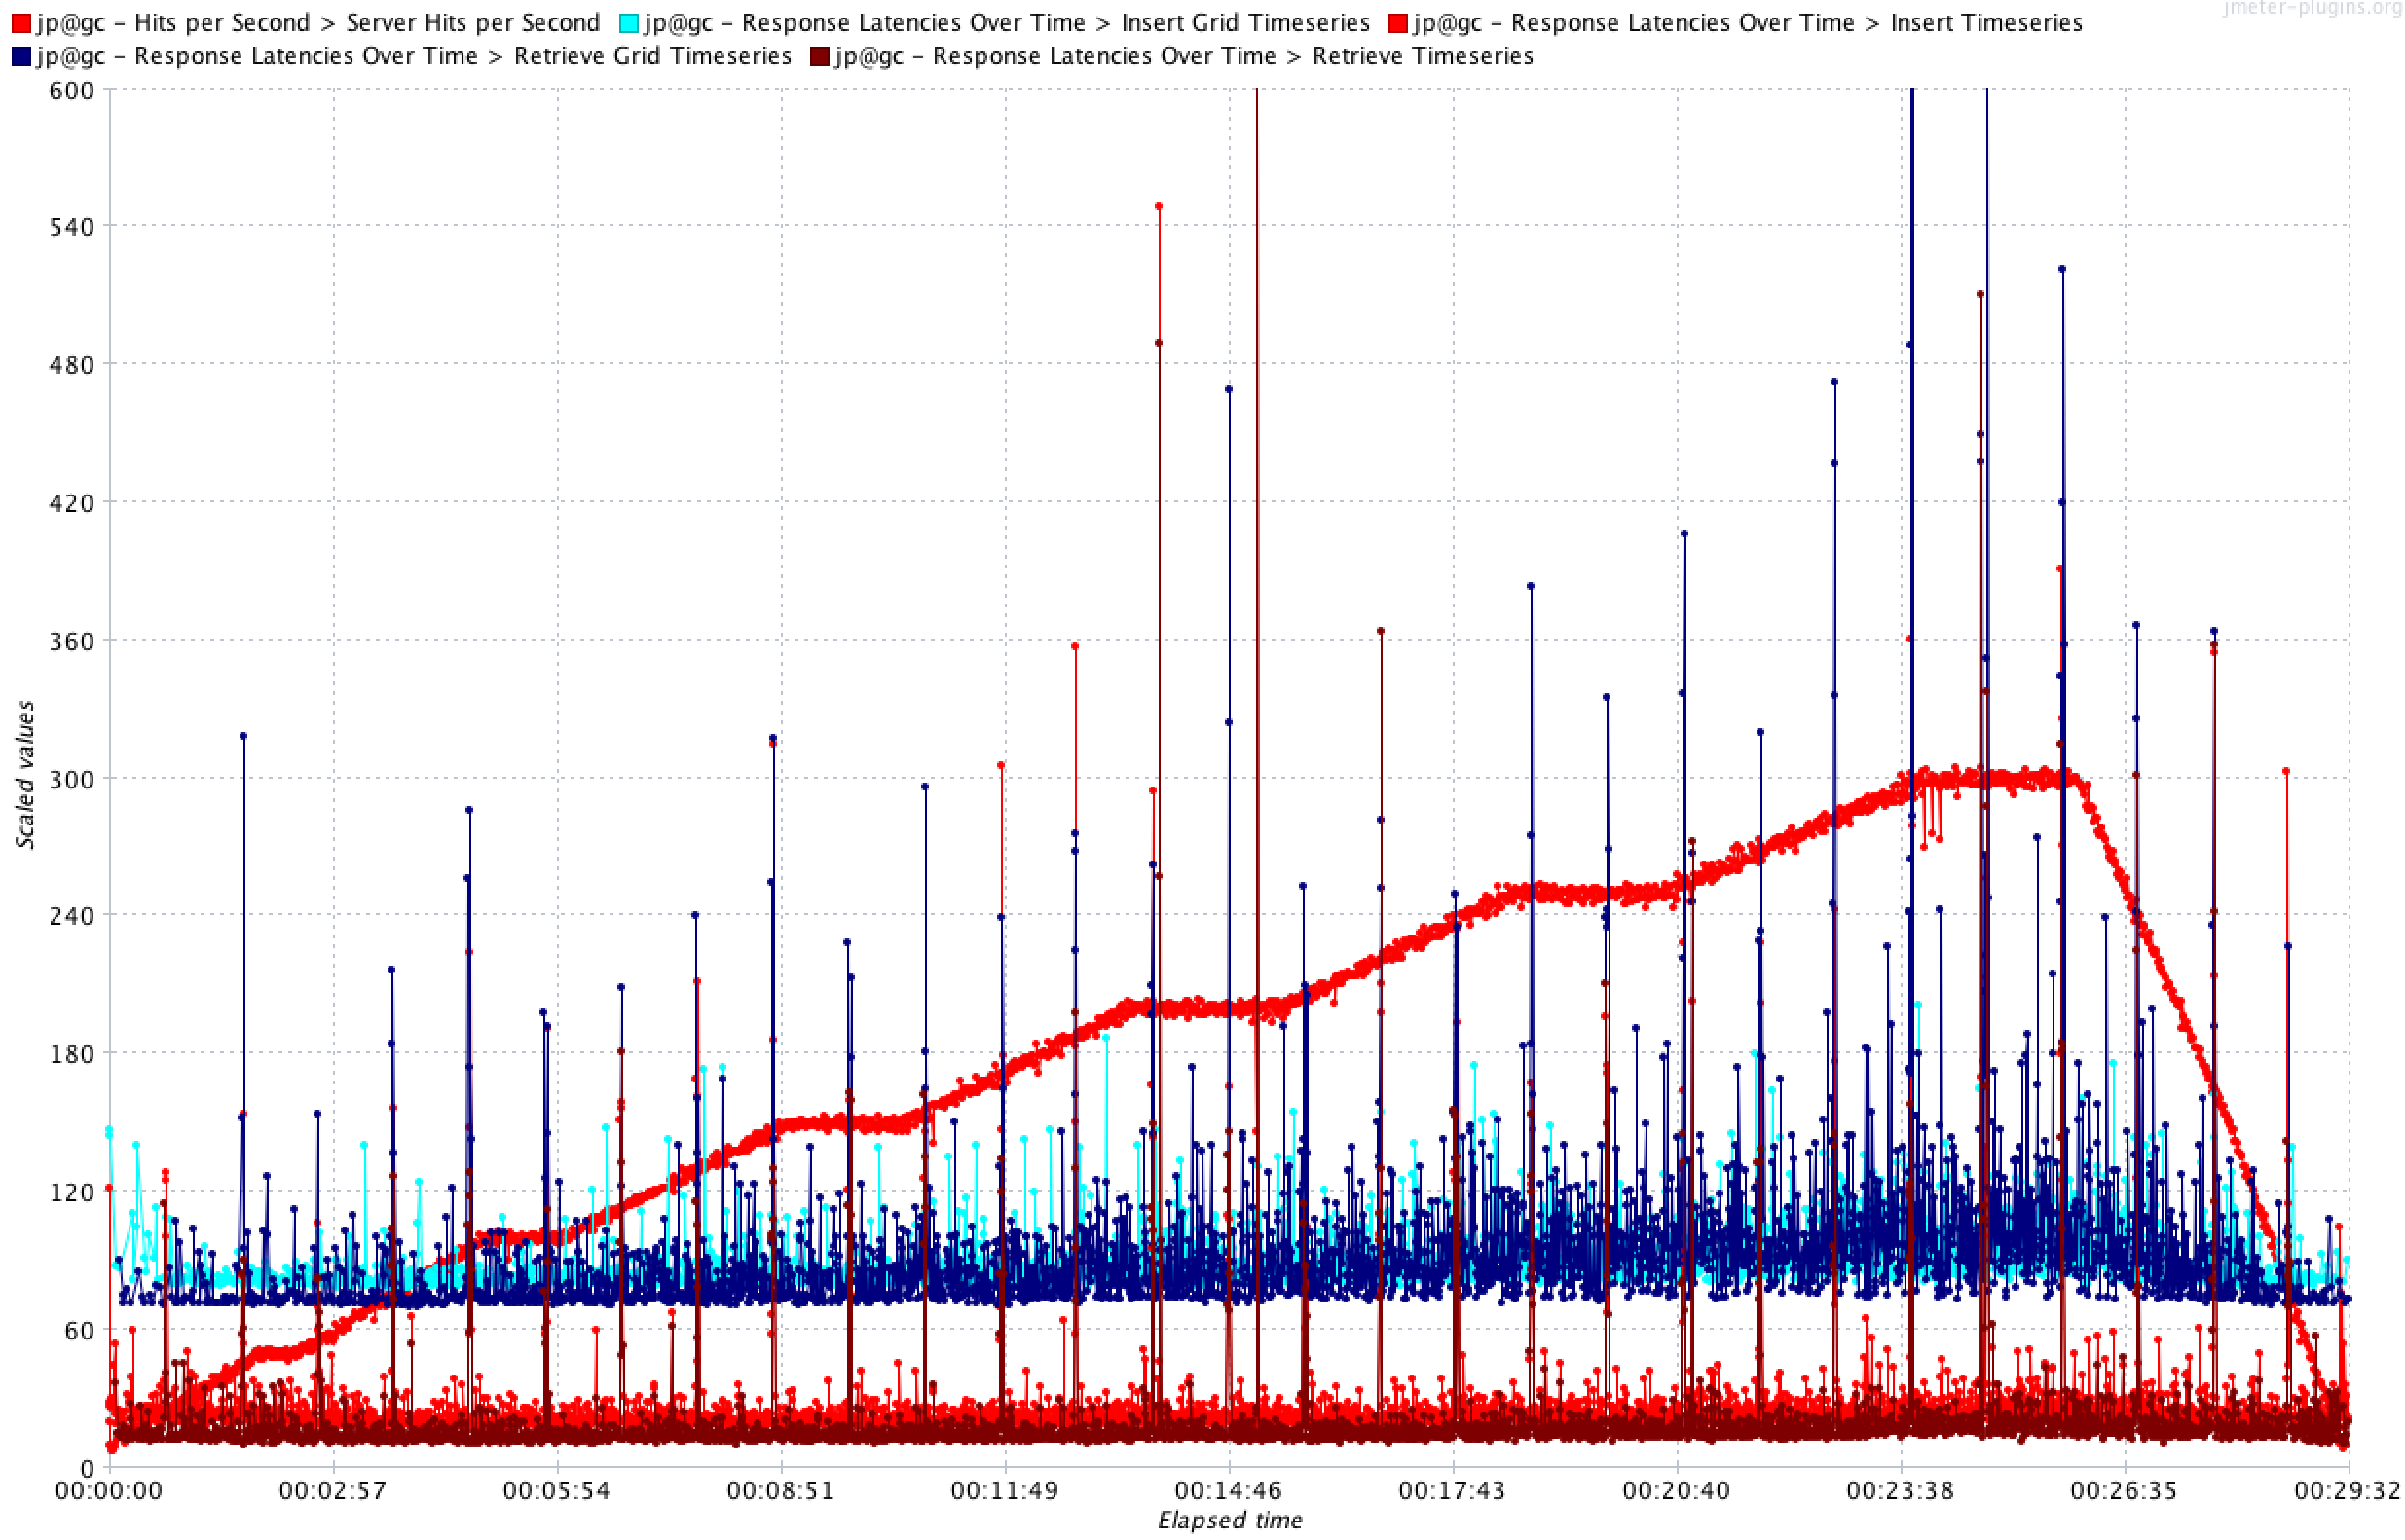
\includegraphics[width=0.8\textwidth]{results/obs/all/obs_all_15m_res_latencies_against_hits.png}
    \caption{Performance Test - Latency against server hits}
    \label{fi:test_obs_all_15m_latency}
\end{figure}
\ref{fi:test_obs_all_15m_latency} graph provides a overview of the variation of latency over elapsed time of the test plan against number of server hits per second for 15min data.
This graph show that over the time \acrshort{wdias} were able to keep the latency constant over the test plan. But at the peak time, it tend to vary from the mean value a lot.
One noticeable fact is, throw out the test time period, it shows spikes in latency when compared to \ref{fi:test_obs_all_60m_latency} and \ref{fi:test_obs_all_30m_latency}.

\begin{figure}[htp]
    \centering
    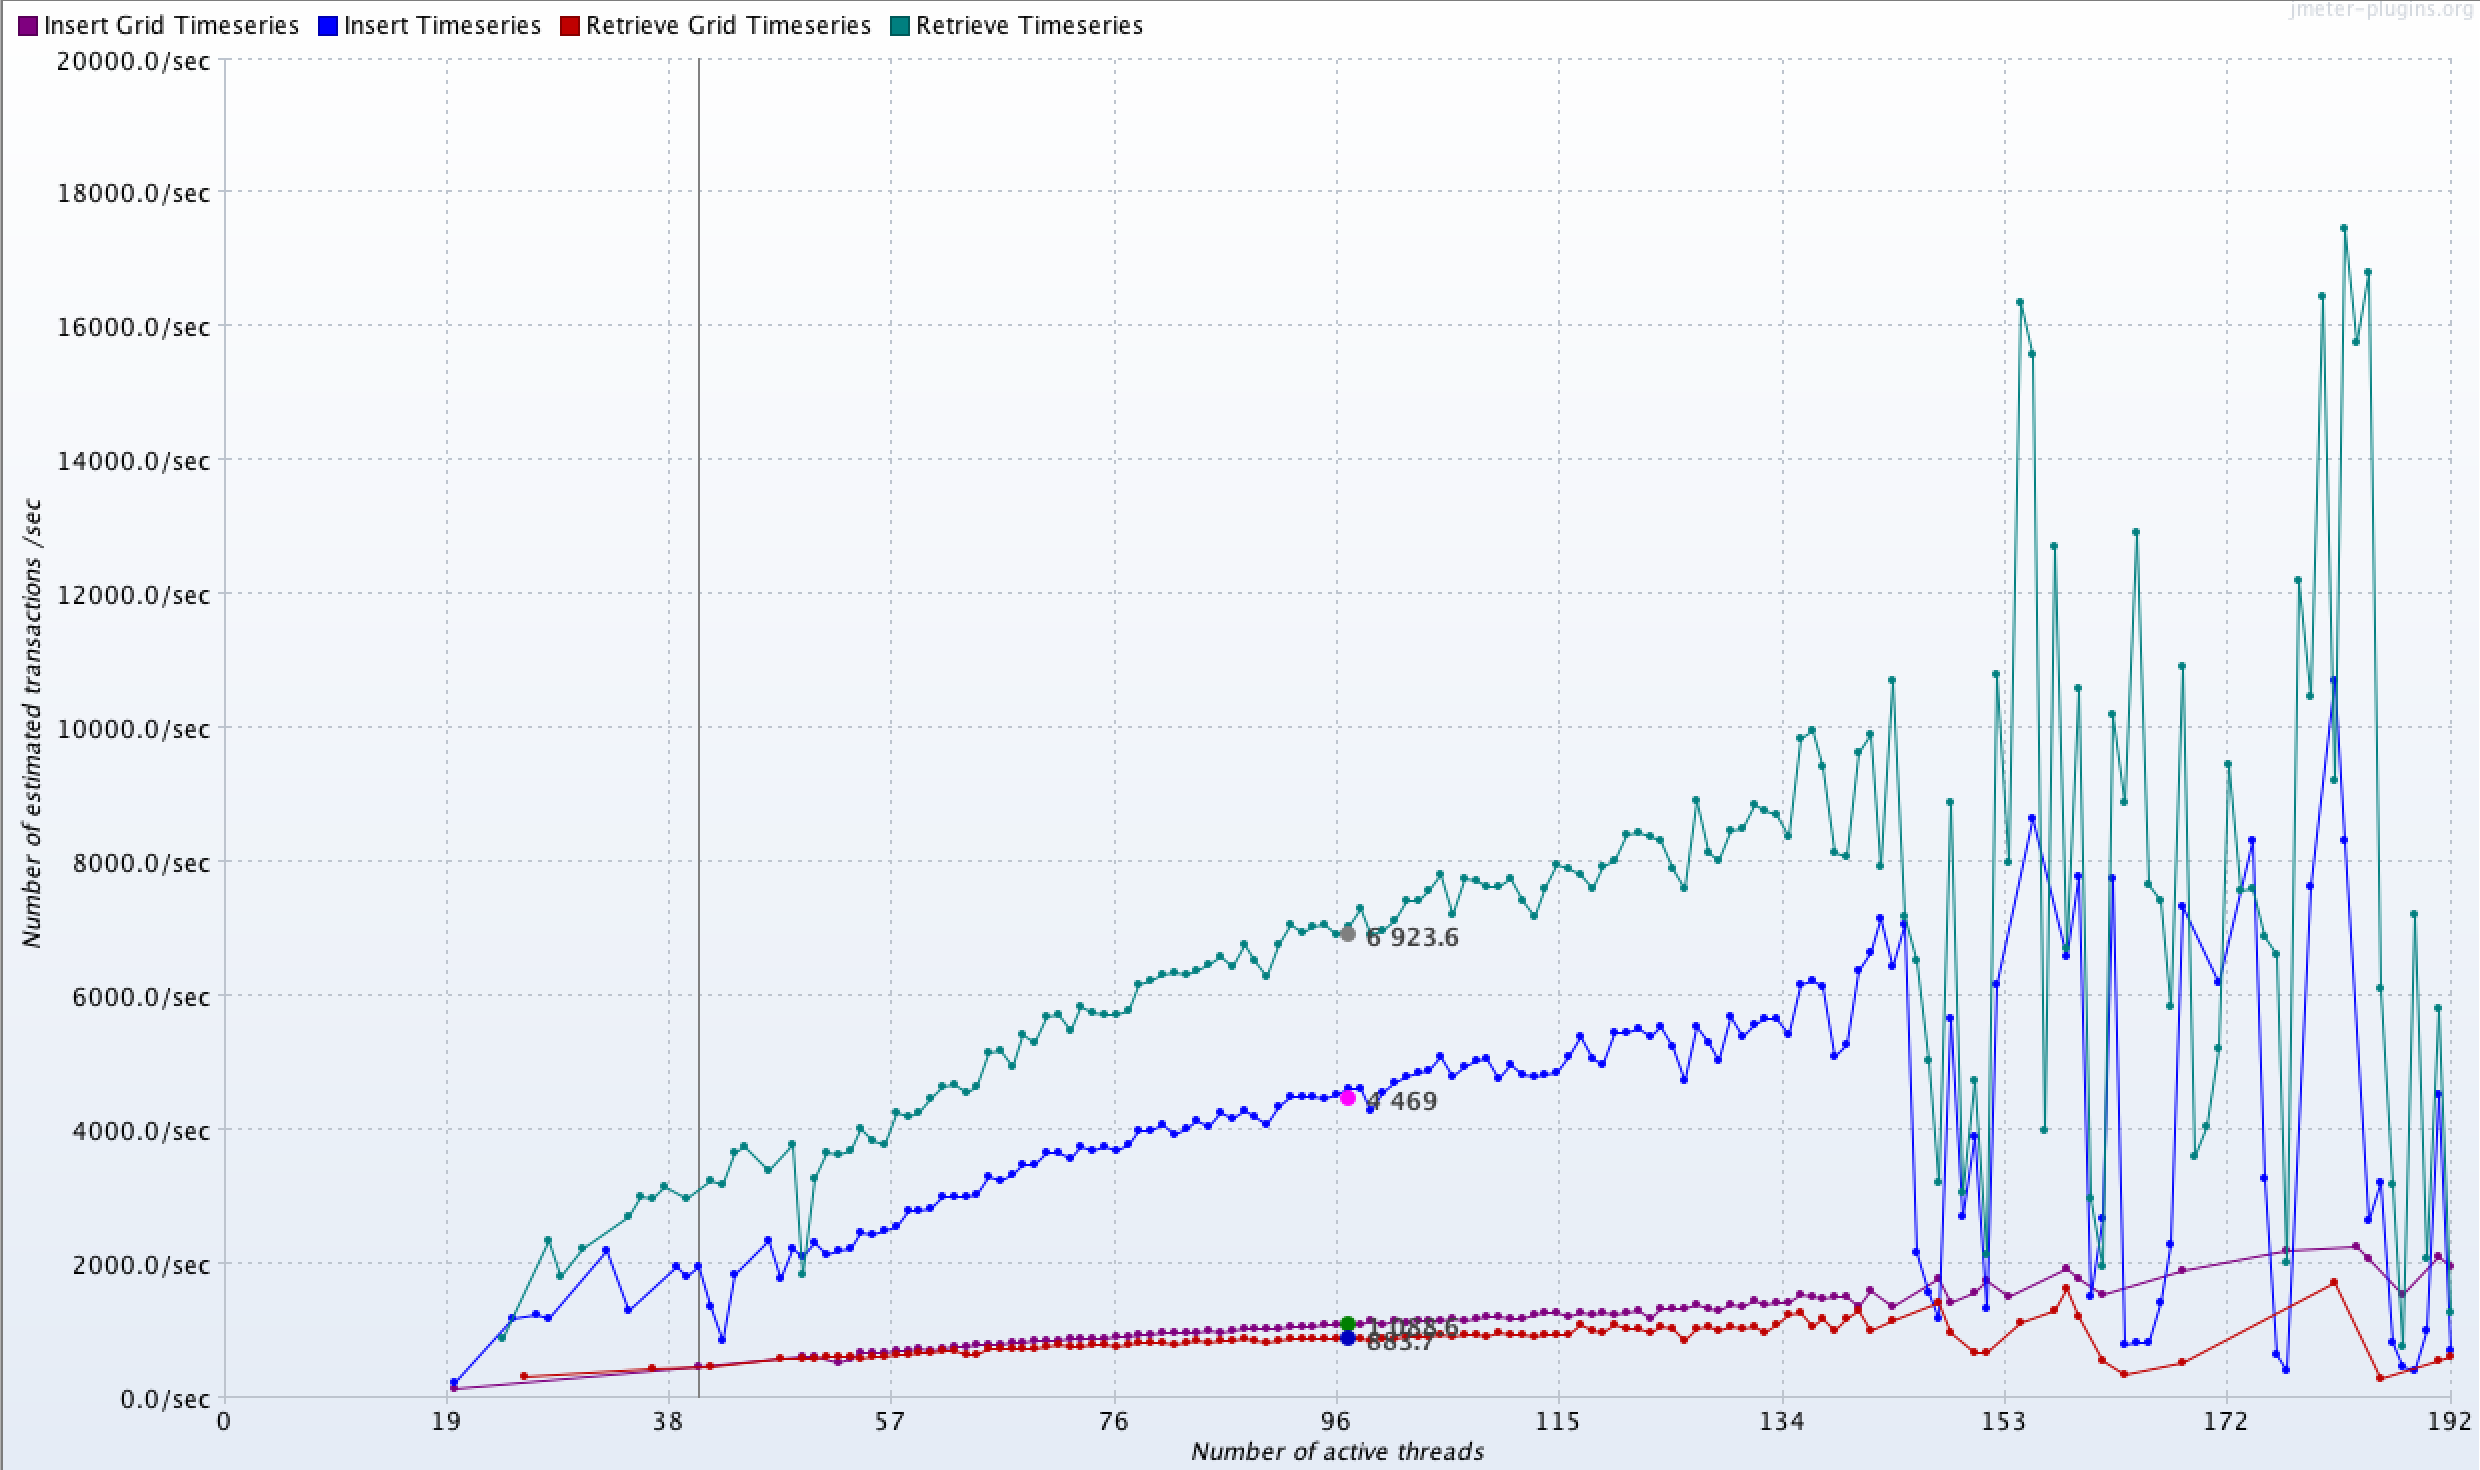
\includegraphics[width=0.8\textwidth]{results/obs/all/obs_all_15m_transaction_throughtput_vs_threads.png}
    \caption{Performance Test - Transaction Throughput vs Threads}
    \label{fi:test_obs_all_15m_throughtput}
\end{figure}
\ref{fi:test_obs_import_15m_throughtput} shows the total server's transaction throughput against number of active threads.
The formula for total server transaction throughput is \(<active threads> * 1 second / <1  thread response time>\) \cite{JMeterPluginsDocumentationJMeter-Plugins.org}. Basically, it shows the statistical maximum possible number of transactions based on number of users accessing the application.
With combining the \ref{fi:test_obs_all_15m_latency}, this graph show that the throughput of the system get increased without much change in the latency, thus it proves the scalability of the \acrshort{wdias}.

\begin{figure}[htp]
    \centering
    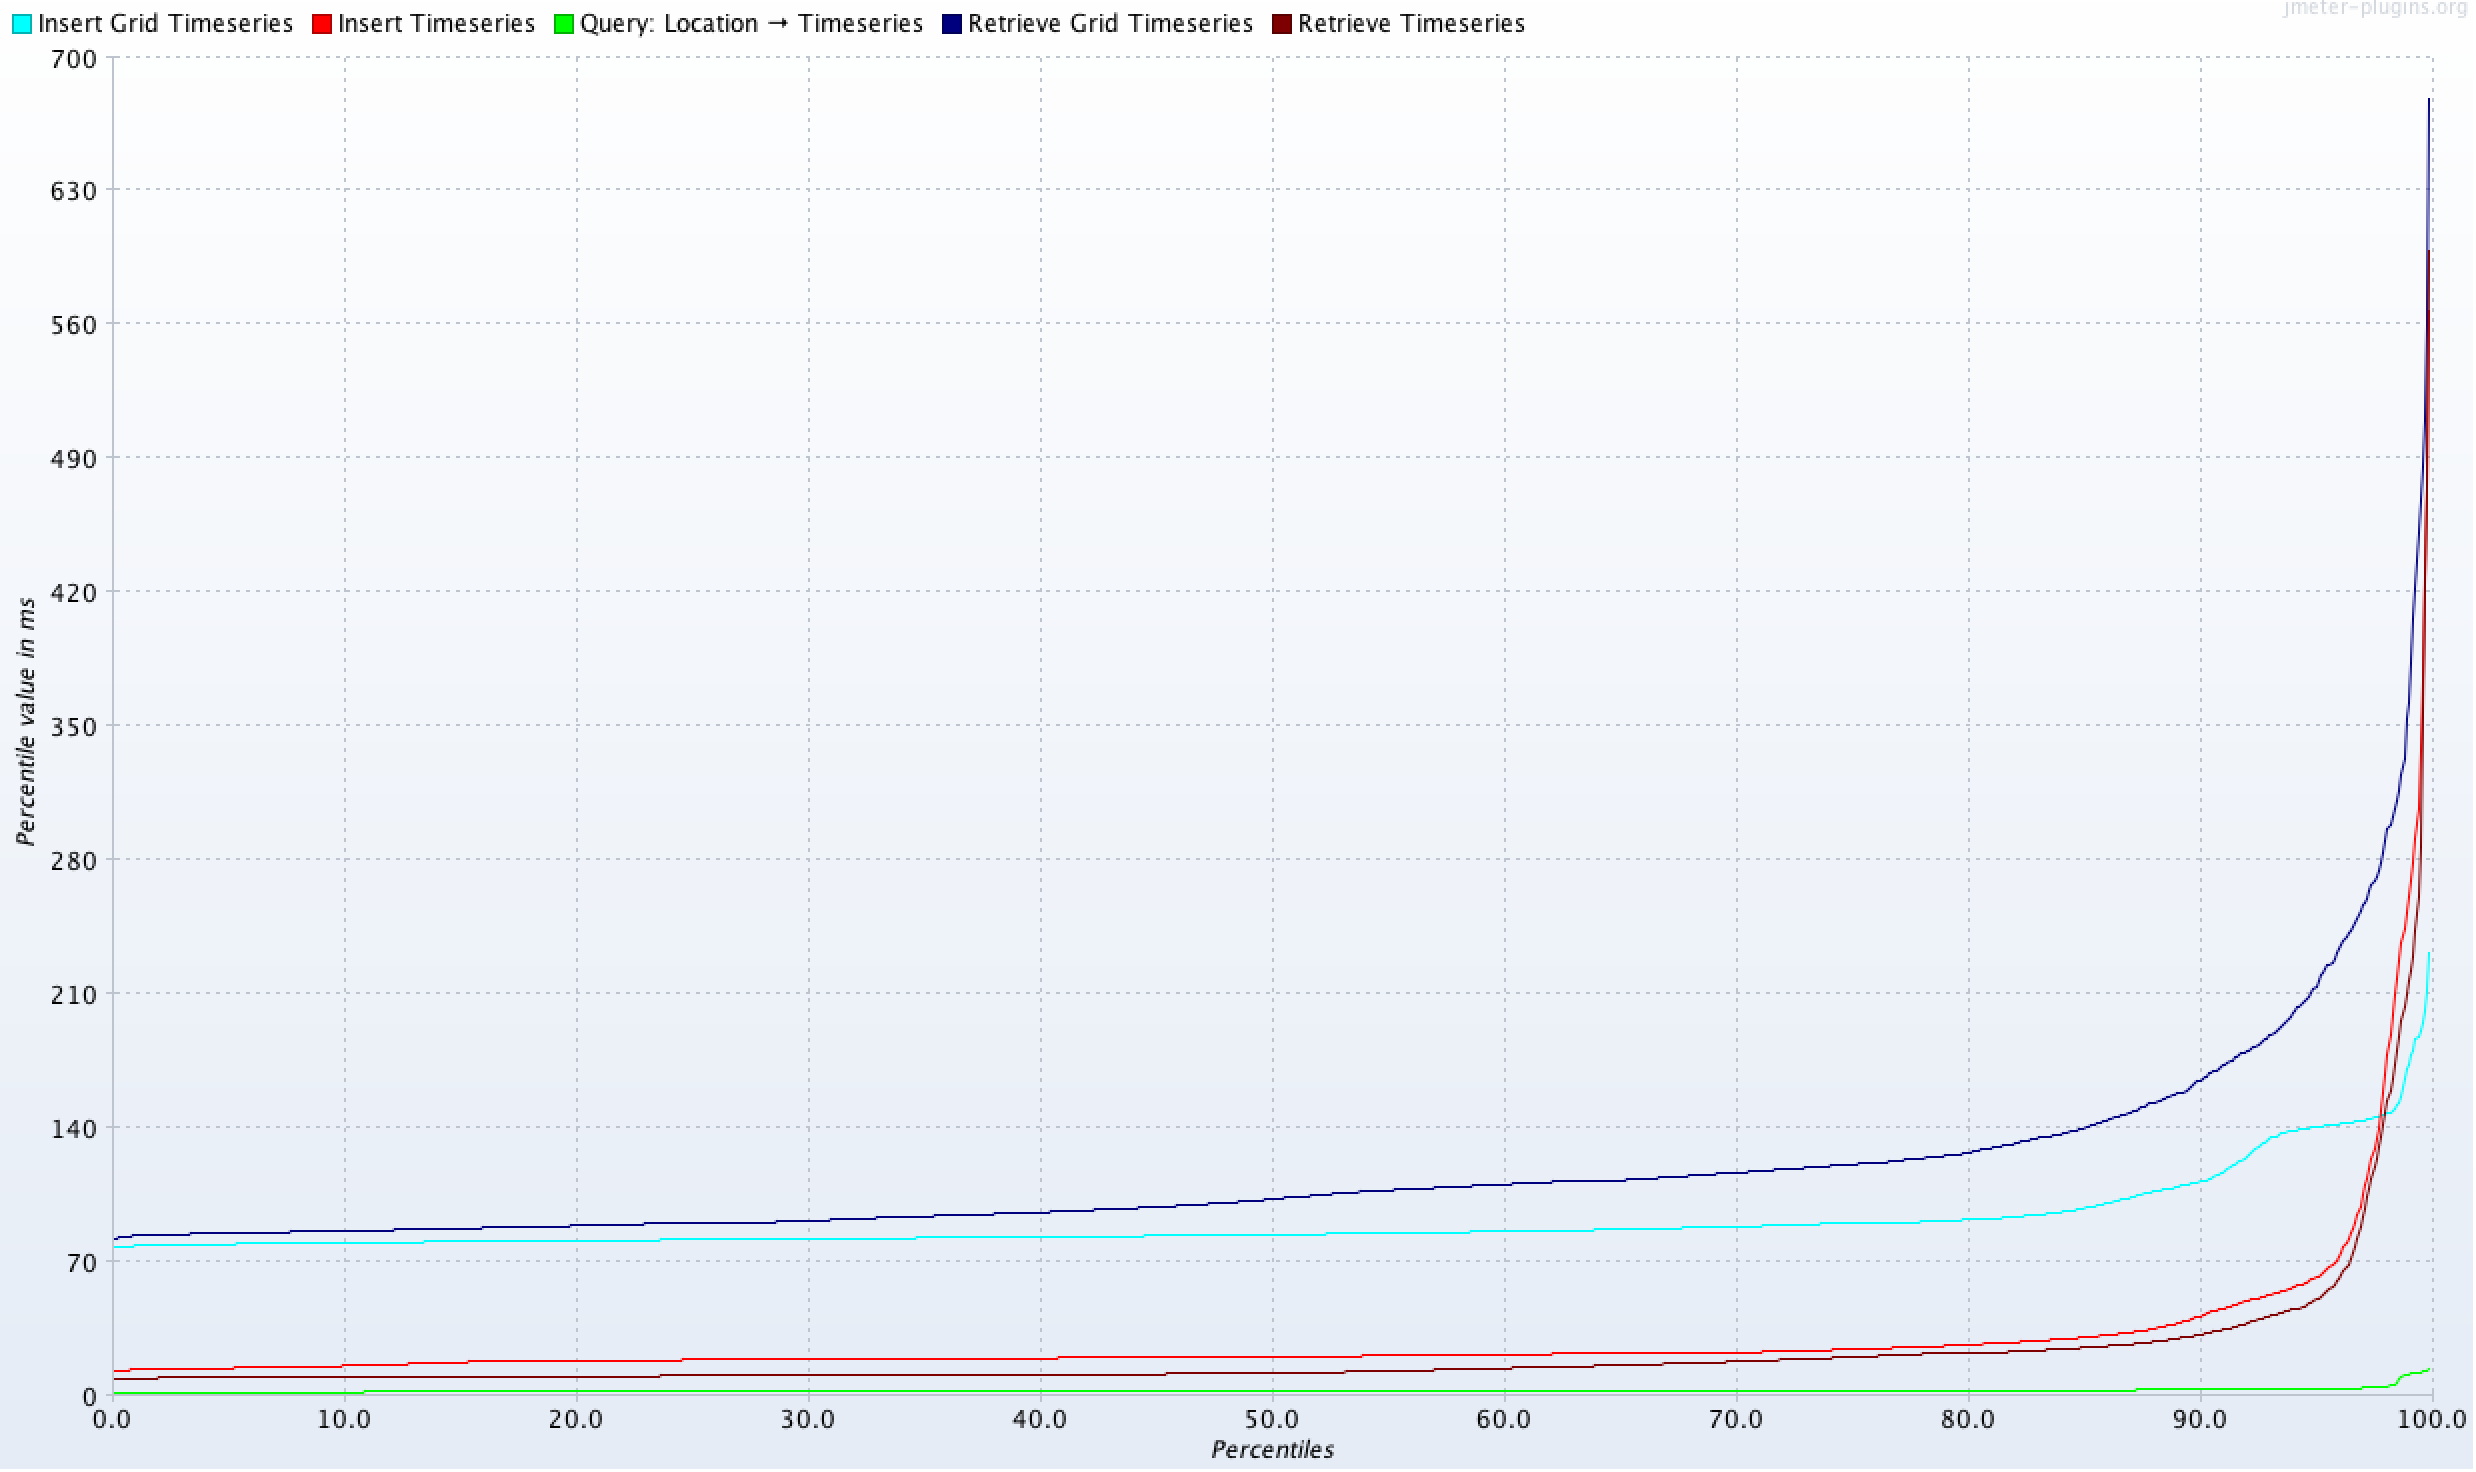
\includegraphics[width=0.8\textwidth]{results/obs/all/obs_all_15m_response_times_percentiles.png}
    \caption{Performance Test - Response times Percentiles}
    \label{fi:test_obs_all_15m_latency_percentile}
\end{figure}
\ref{fi:test_obs_all_15m_latency_percentile} visually shows the summary of \ref{tab:obs_all_15_min_summary} latency up to 90\% percentile. With a higher request size data, the \acrshort{wdias} able to process the requests without significant change in latency up to 90\% percentile.



\subsection{Full Load test with \acrfull{k8s} auto pod scaling}
\label{subse:obs_test_plan_all_auto_15min}
\begin{figure}[htp]
    \centering
    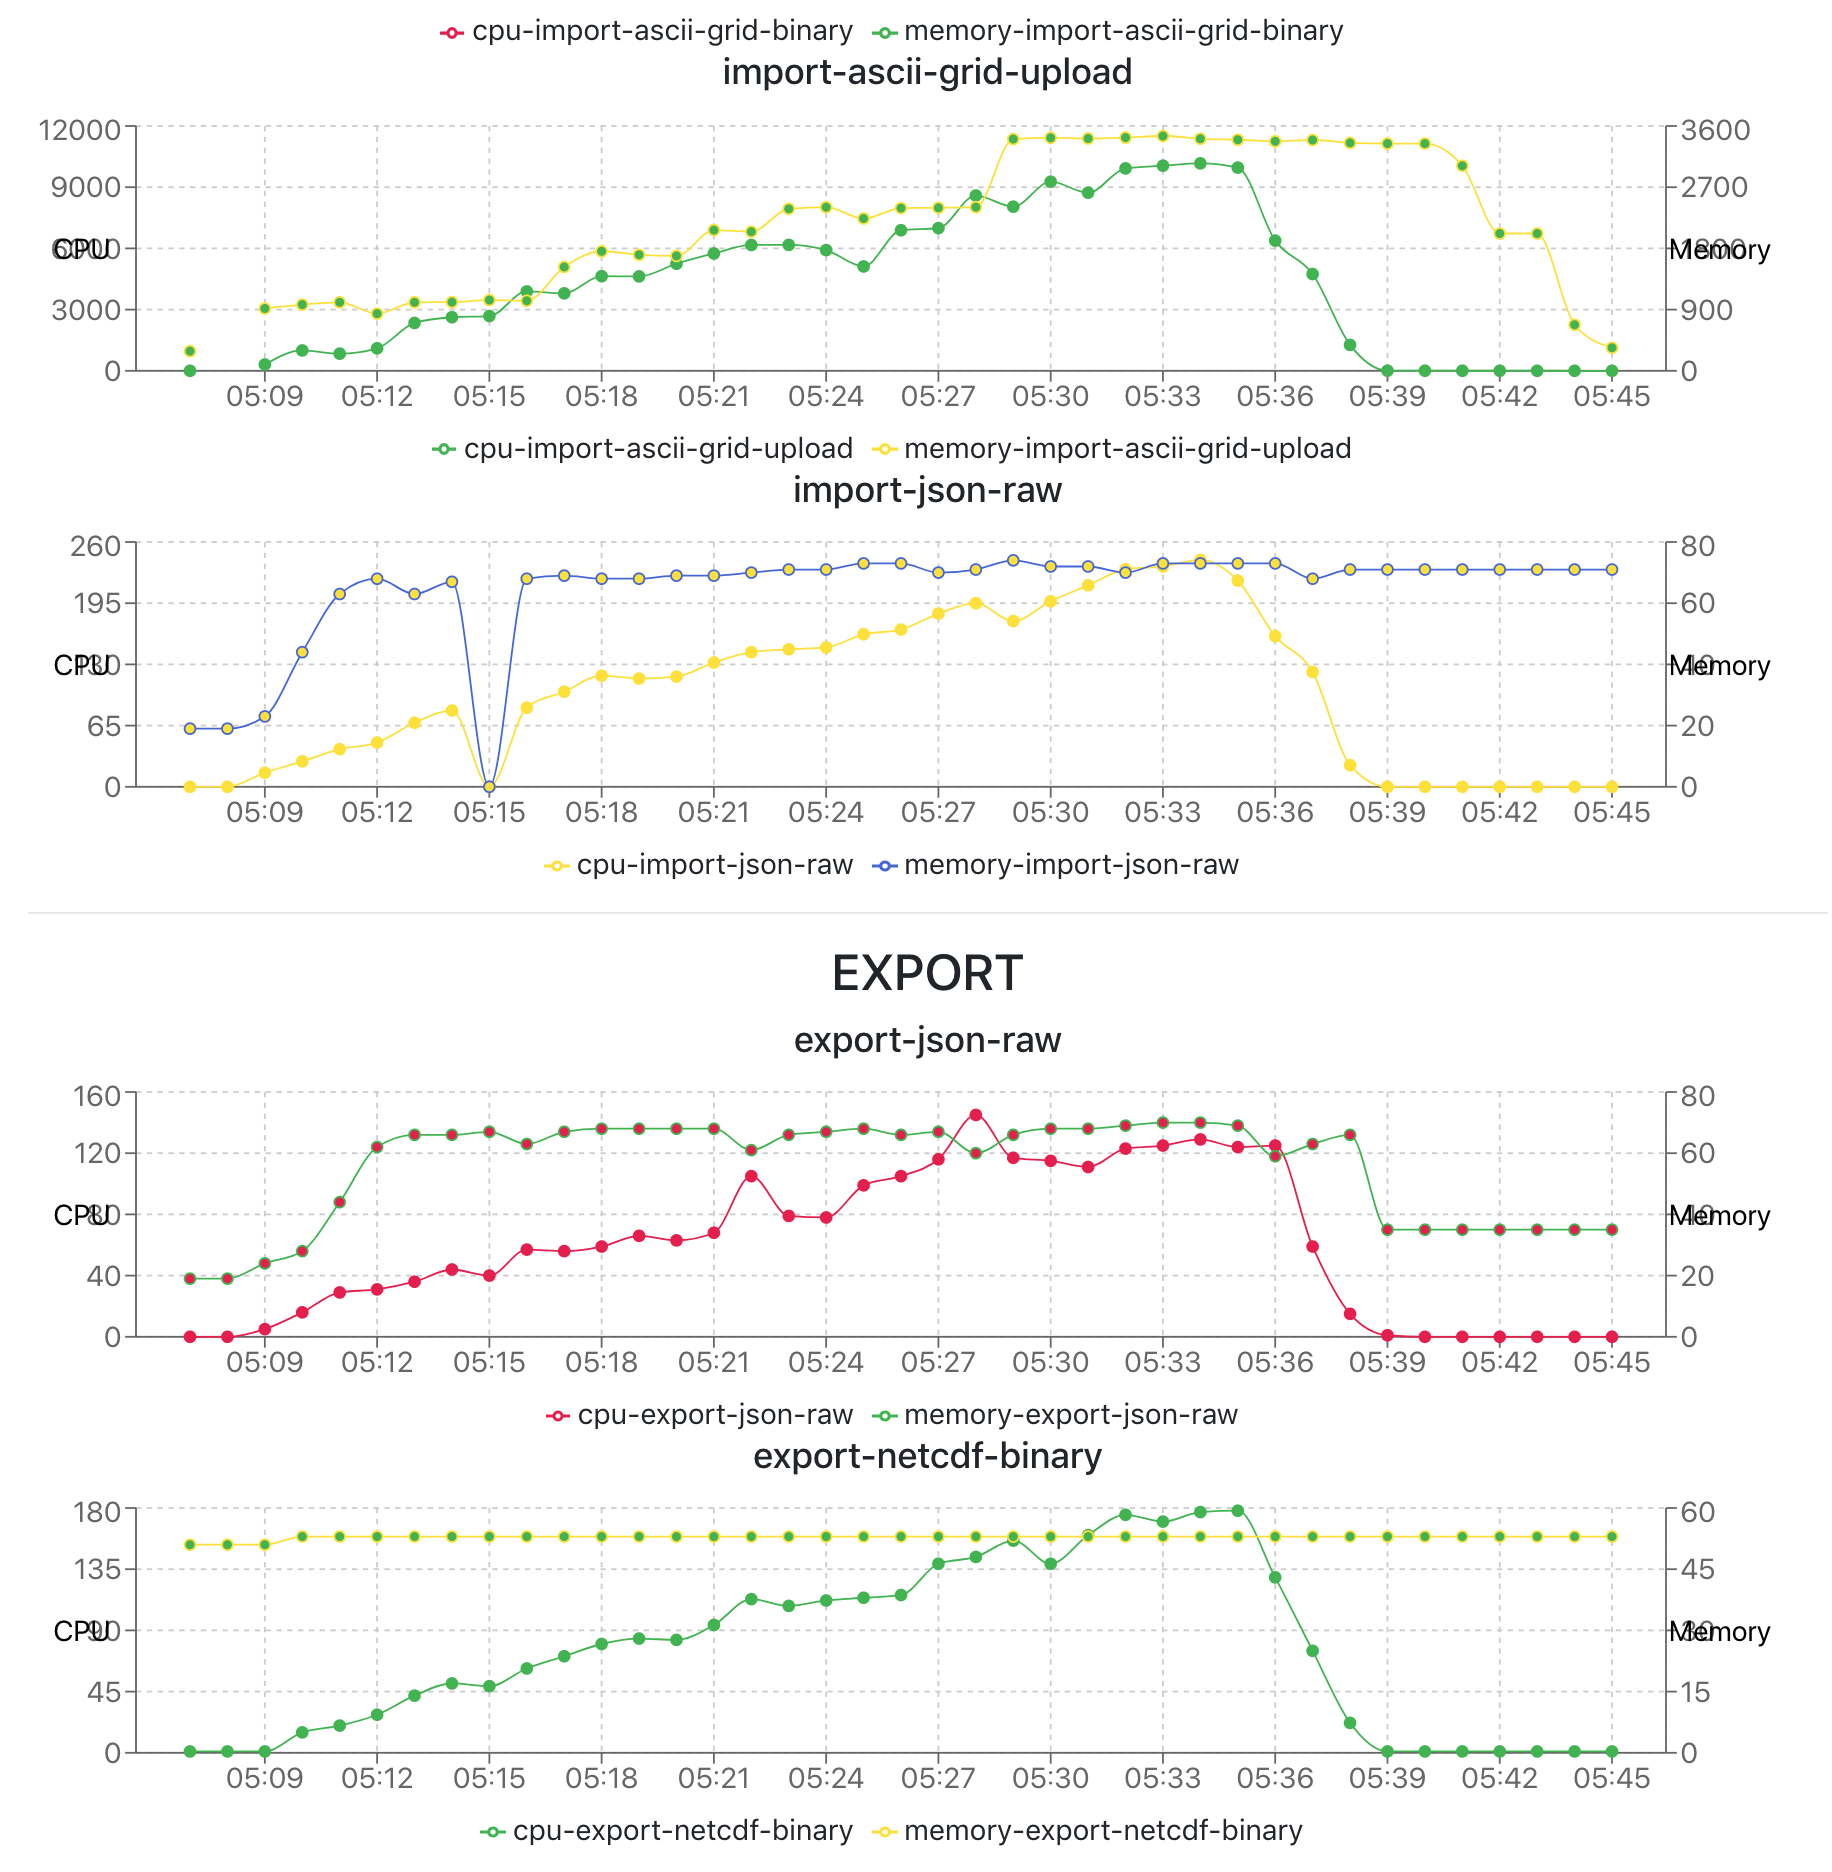
\includegraphics[width=0.8\textwidth]{results/obs/all_auto/obs_all_auto_15m_import_export_res.png}
    \caption{Performance All Test 15min Interval - Auto Scaling Resource Usage of Import and Export Modules }
    \label{fi:obs_all_auto_15m_import_export_res}
\end{figure}

\begin{figure}[htp]
    \centering
    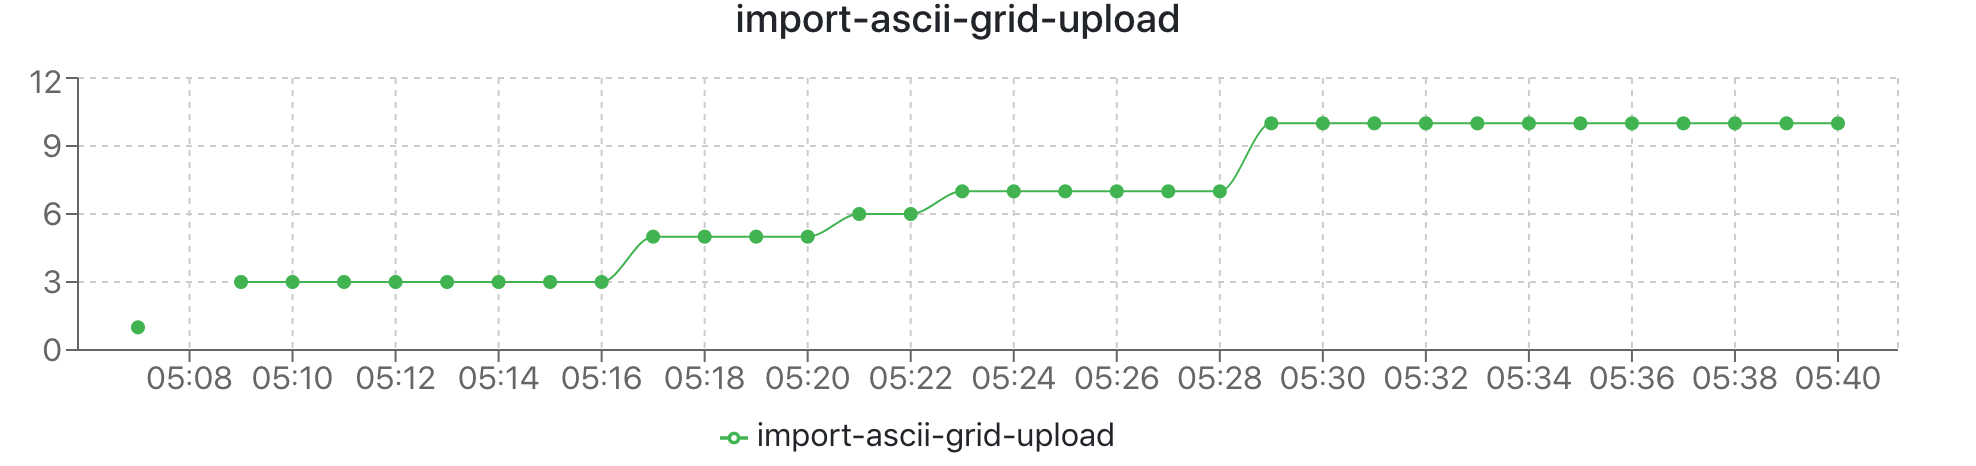
\includegraphics[width=0.8\textwidth]{results/obs/all_auto/obs_all_auto_15m_import_grid_pod.png}
    \caption{Performance All Test 15min Interval - Auto Scaling Import ASCII Grid Number of Pods Over Time }
    \label{fi:obs_all_auto_15m_import_grid_pod}
\end{figure}

\begin{figure}[htp]
    \centering
    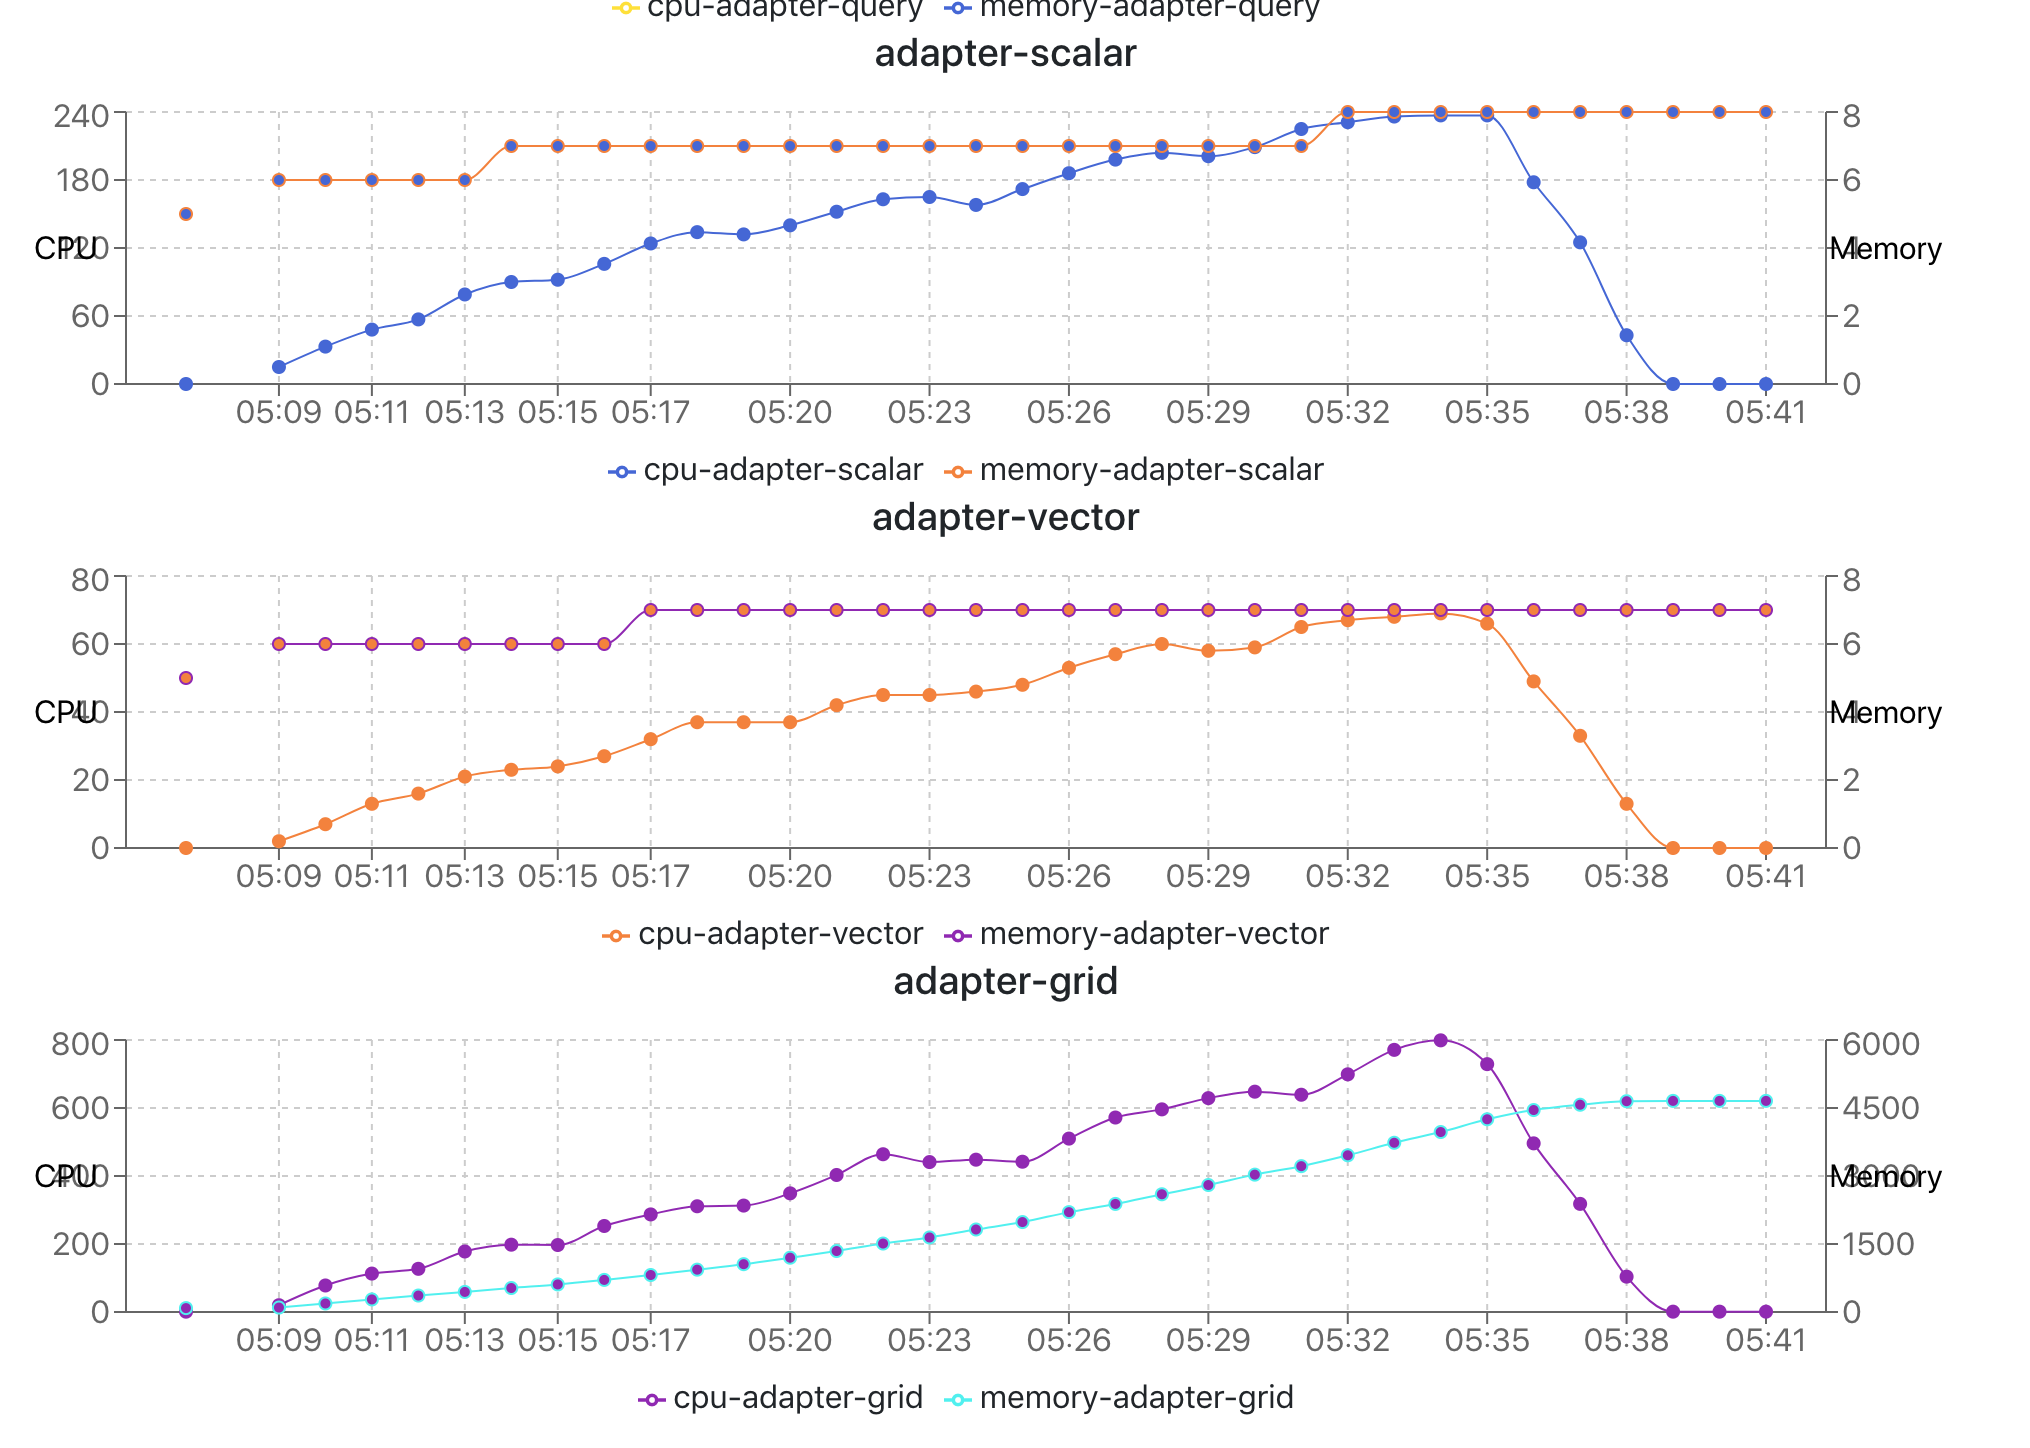
\includegraphics[width=0.8\textwidth]{results/obs/all_auto/obs_all_auto_15m_adapter_dbs_res.png}
    \caption{Performance All Test 15min Interval - Auto Scaling Resource Usage of Database Adapters }
    \label{fi:obs_all_auto_15m_adapter_dbs_res}
\end{figure}



\subsection{Import module load test}
\begin{table}[]
\begin{tabulary}{\linewidth}{|L|C|C|C|C|C|C|C|C|}
\hline
Label & \# Samples & Average & Min & Max & 90\% Line & Std. Dev. & Error \% & RPS \\ \hline
Insert Timeseries & 91345 & 212 & 15 & 5288 & 241 & 556.05 & 0.01\% & 123.4 \\ \hline
Insert Grid Timeseries & 10189 & 108 & 76 & 330 & 148 & 30.98 & 0.00\% & 13.8 \\ \hline
\textbf{TOTAL} & 101534 & 202 & 15 & 5288 & 212 & 528.43 & 0.01\% & 137.2 \\ \hline
\end{tabulary}
\caption{Throughput and Latency of Import test cases with 15min data}
\label{tab:obs_import_15_min_summary}
\end{table}

\begin{figure}[htp]
    \centering
    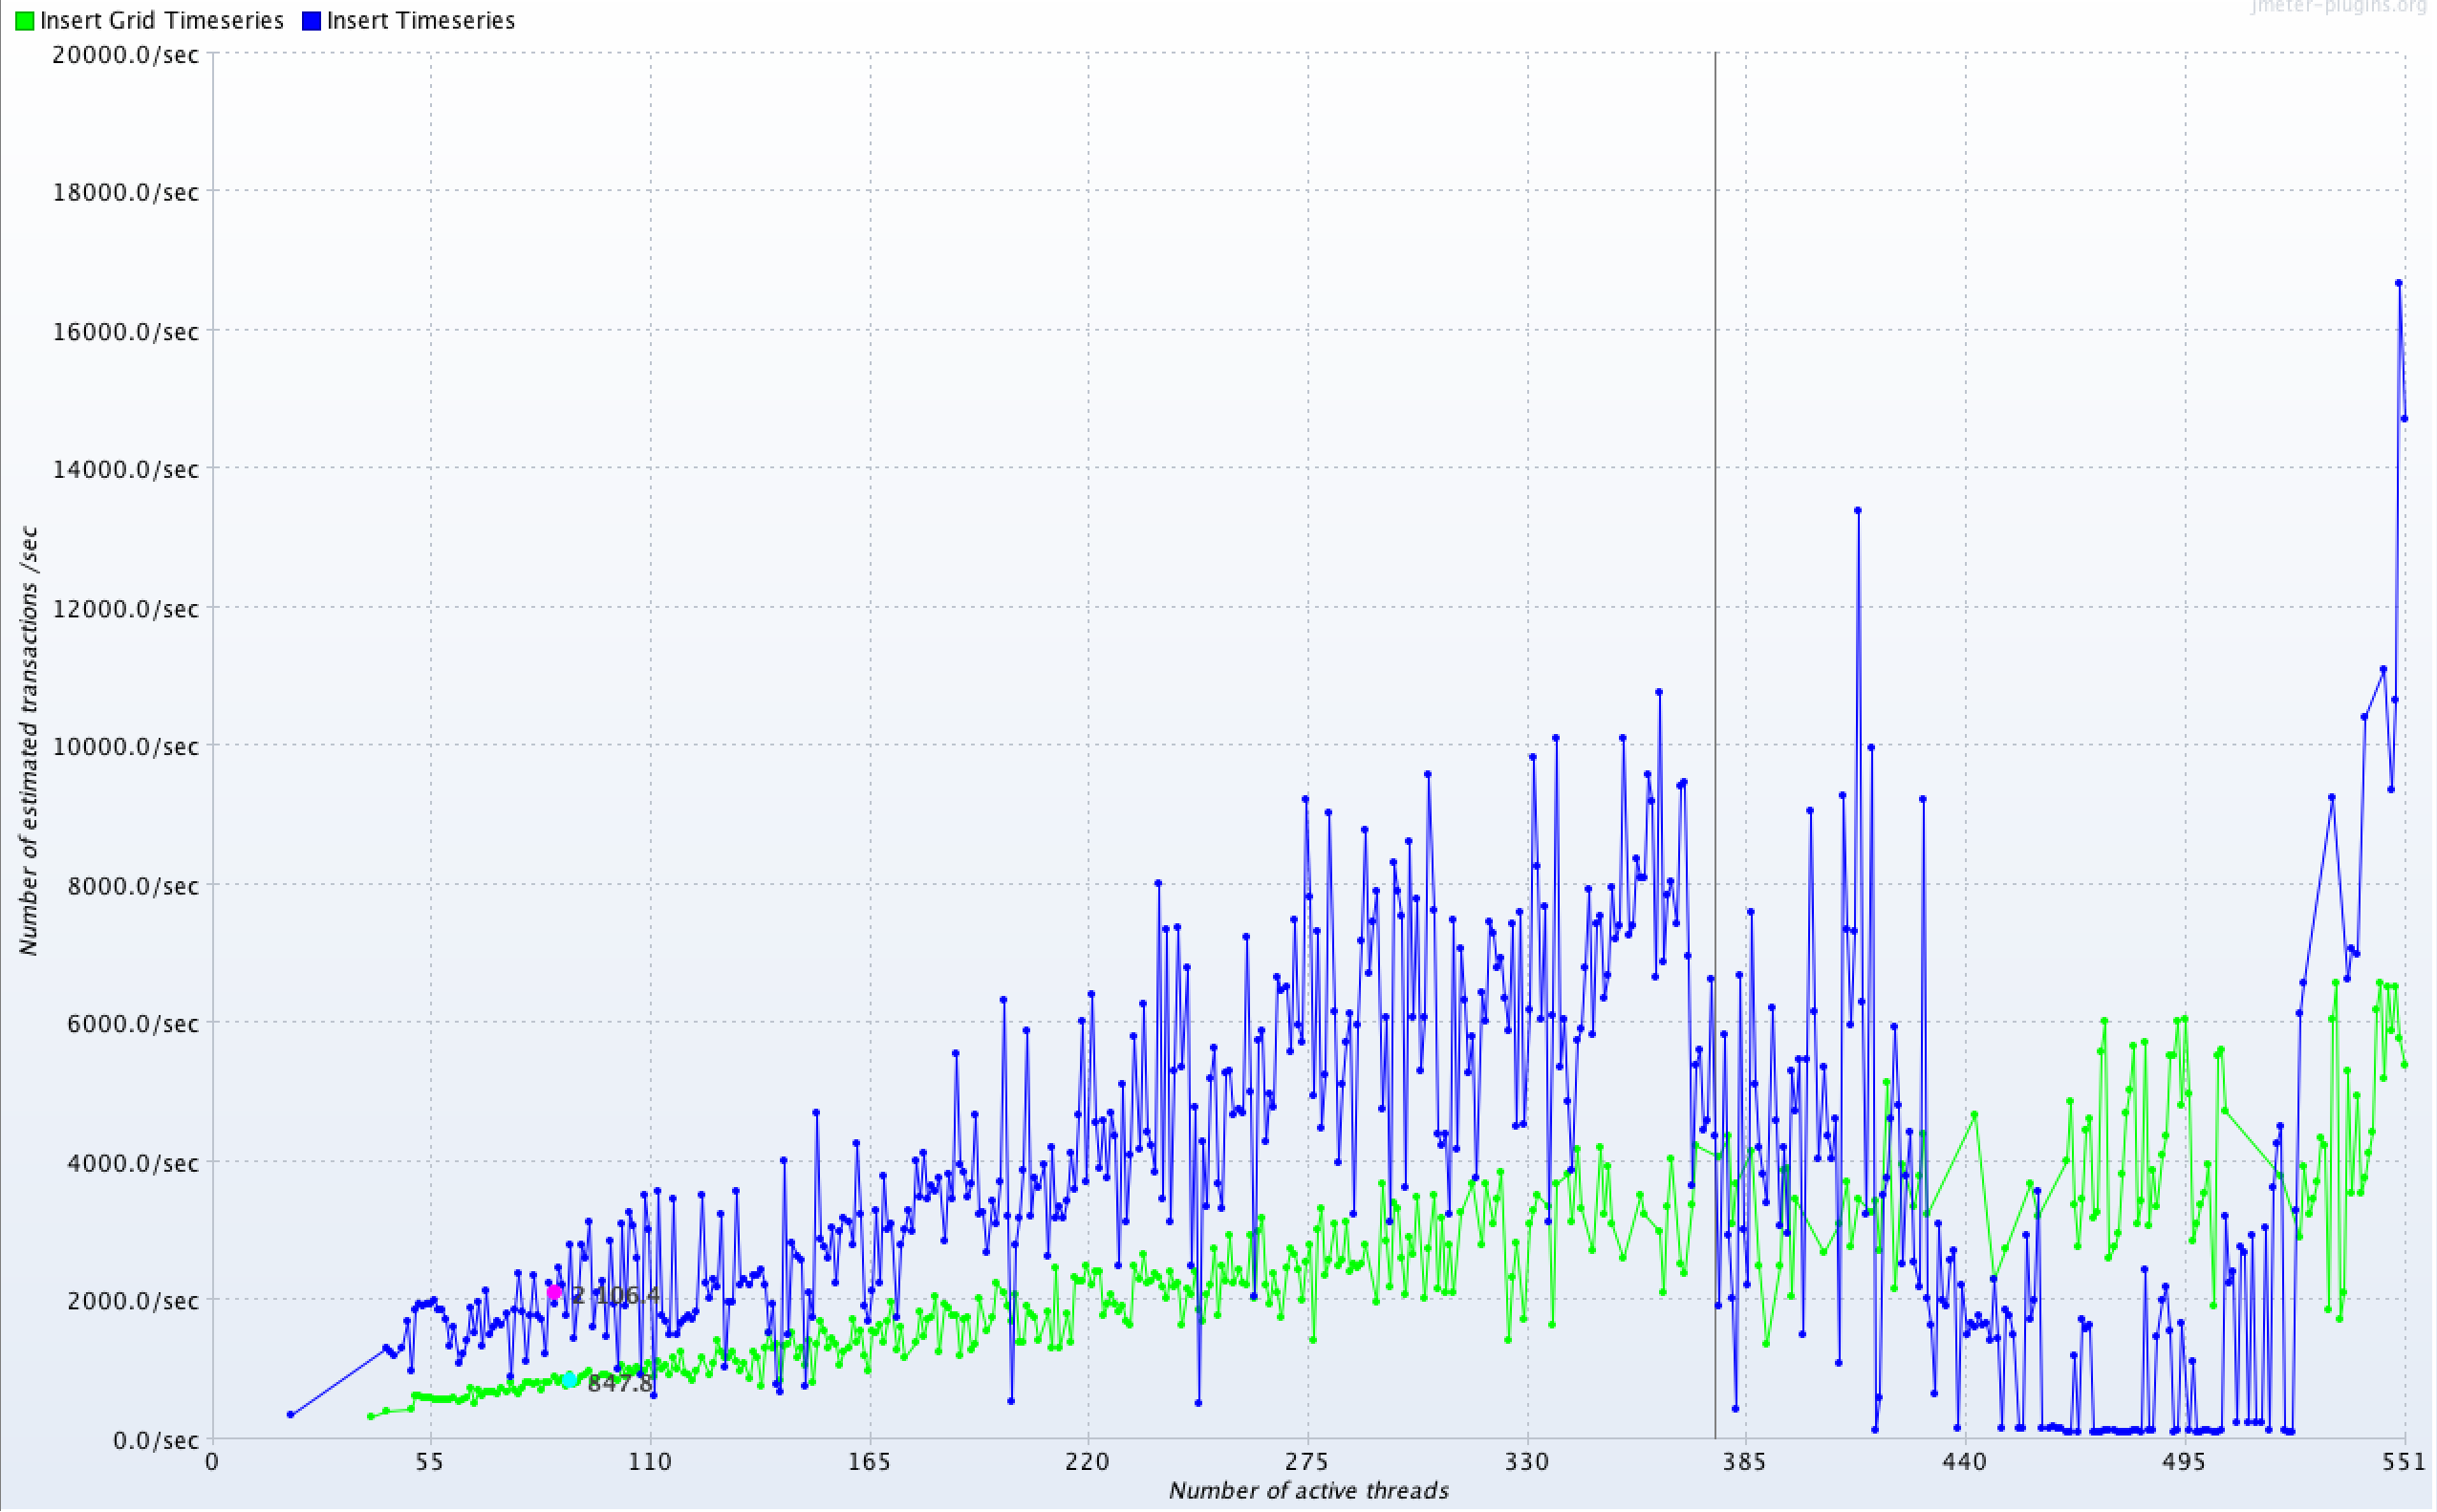
\includegraphics[width=0.8\textwidth]{results/obs/import/obs_import_15m_transaction_throughtput_vs_threads.png}
    \caption{Performance Import Test 15 minutes Interval - Transaction Throughput vs Threads}
    \label{fi:test_obs_import_15m_throughtput}
\end{figure}

\begin{figure}[htp]
    \centering
    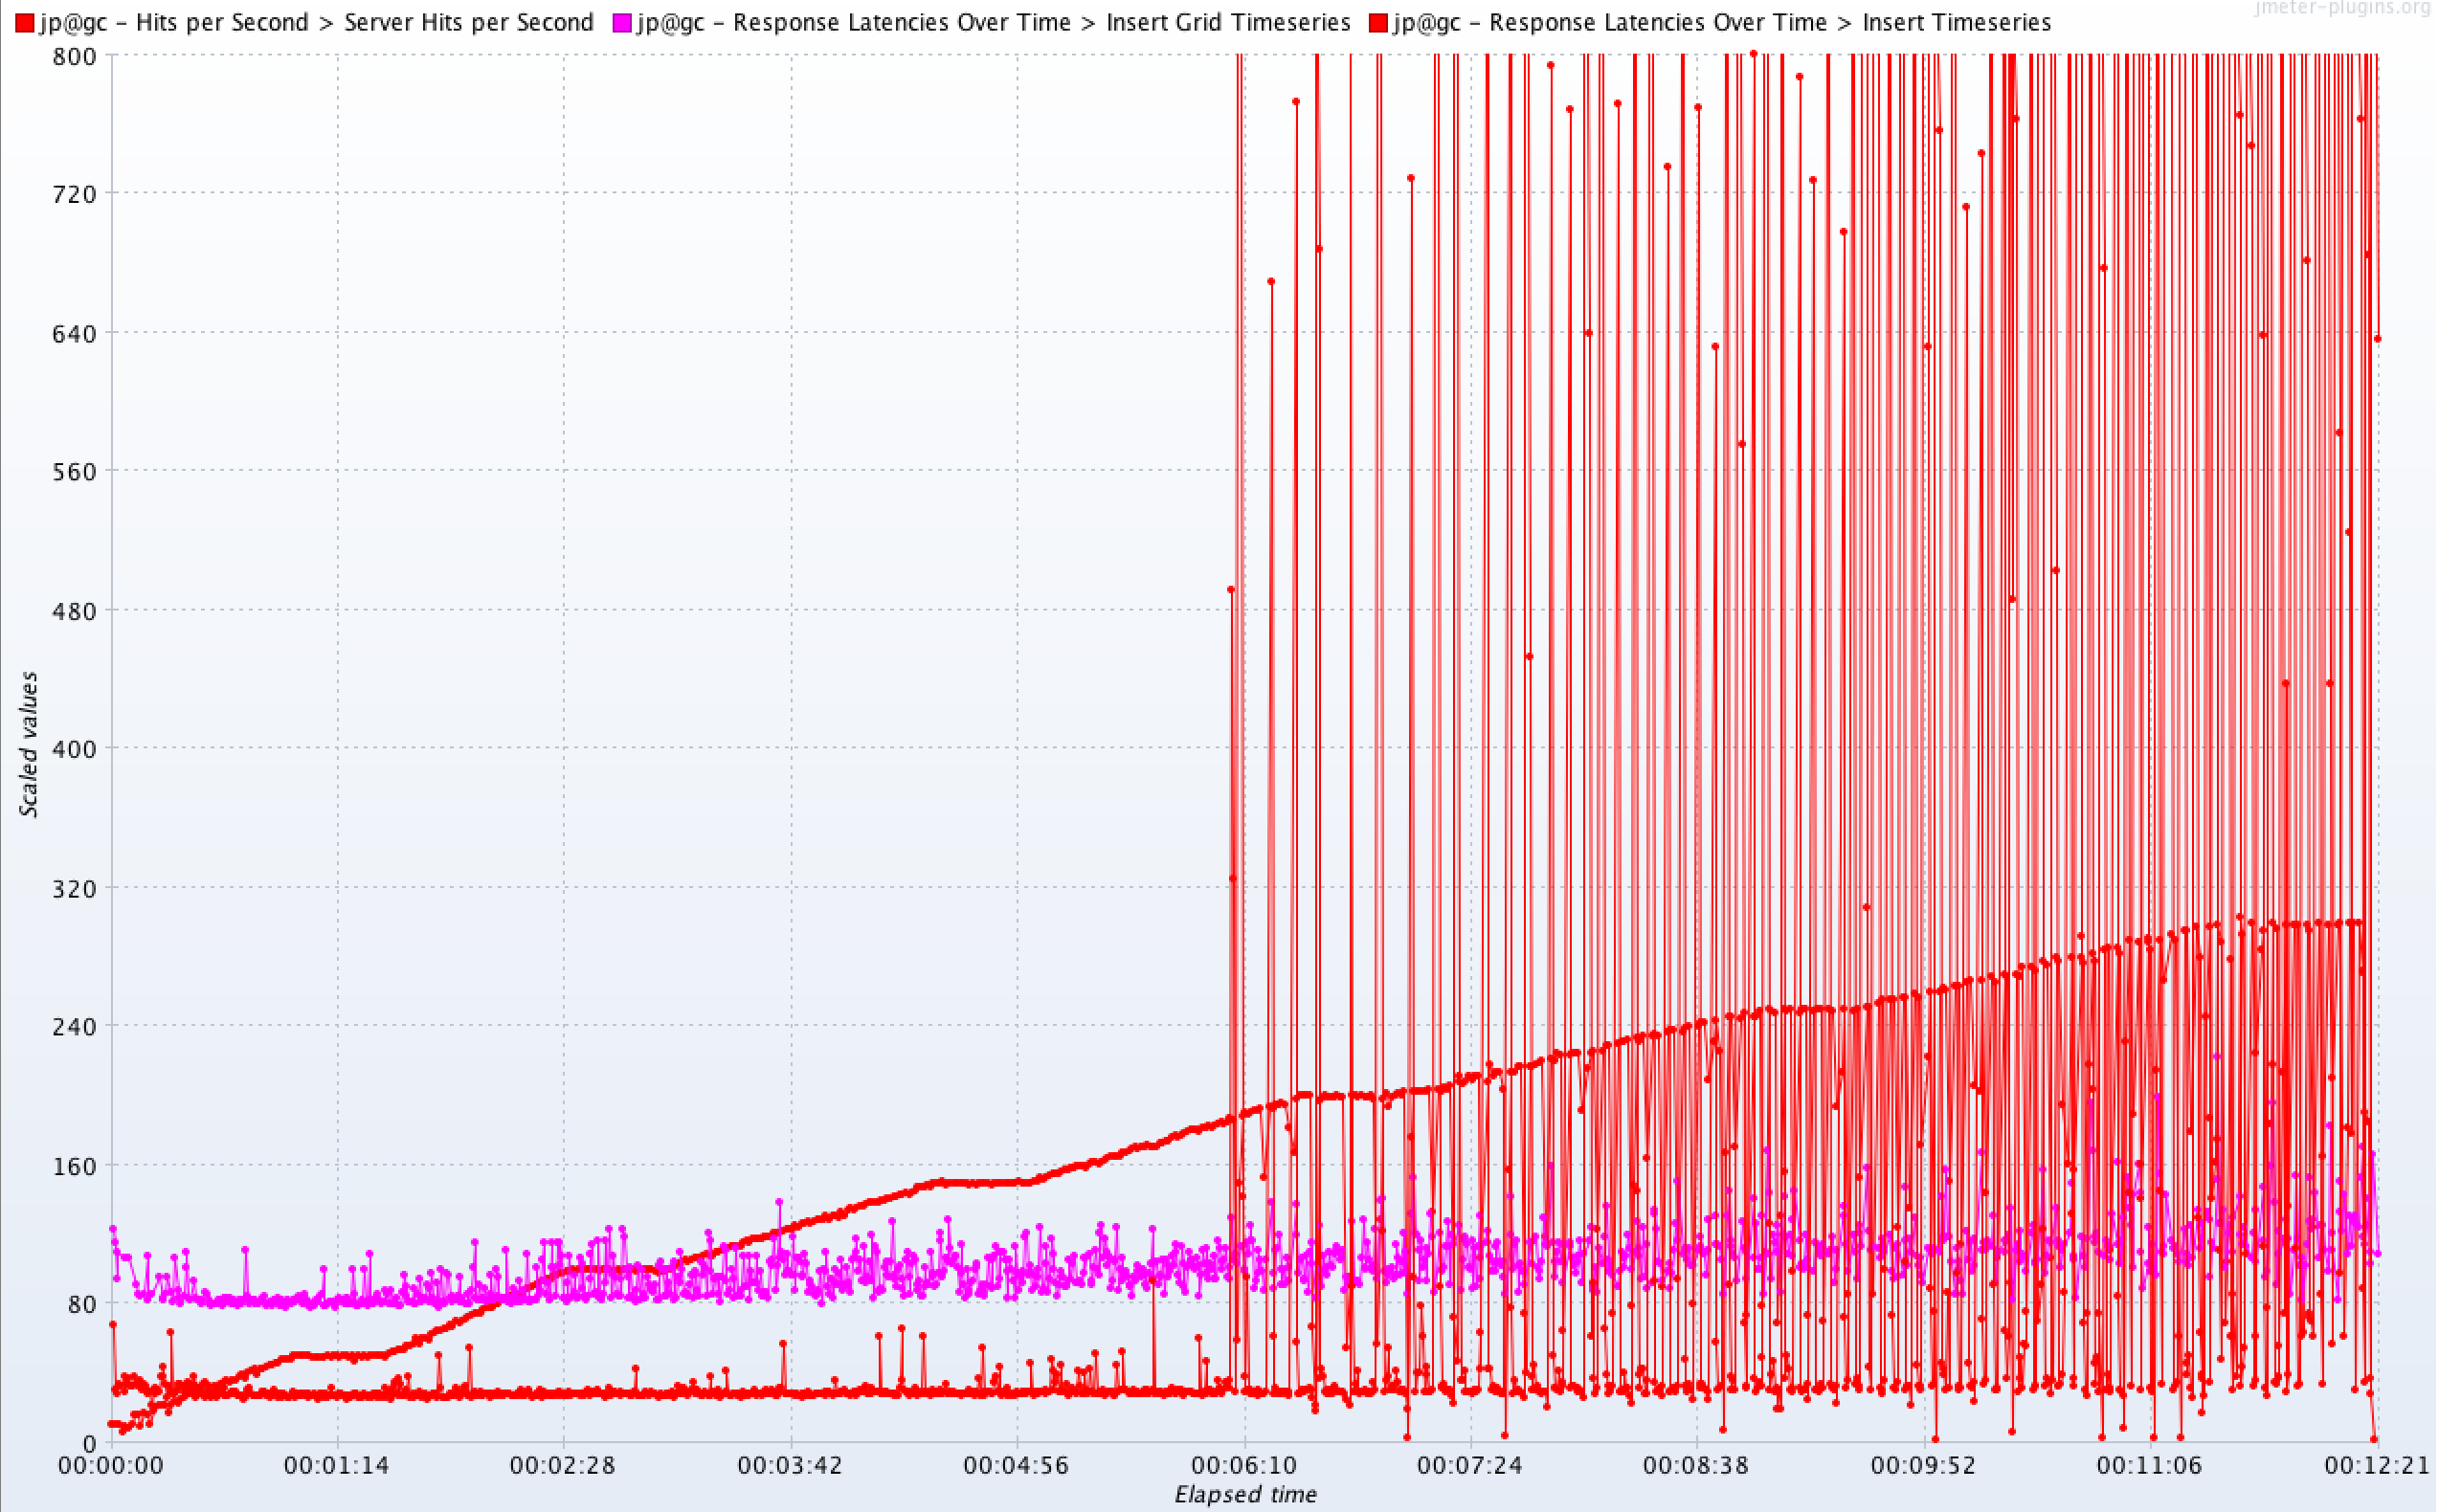
\includegraphics[width=0.8\textwidth]{results/obs/import/obs_import_15m_res_latencies_against_hits.png}
    \caption{Performance Import Test 15 minutes Interval - Latency against server hits}
    \label{fi:test_obs_import_15m_latency}
\end{figure}



\subsection{Export module load test}
Need to redo just after the import
\begin{table}[]
\begin{tabulary}{\linewidth}{|L|C|C|C|C|C|C|C|C|}
\hline
Label & \# Samples & Average & Min & Max & 90\% Line & Std. Dev. & Error \% & RPS \\ \hline
Retrieve Timeseries & 136310 & 9 & 7 & 287 & 11 & 6.37 & 0.00\% & 156.1 \\ \hline
Retrieve Grid Timeseries & 15147 & 265 & 10 & 4044 & 488 & 691.69 & 46.36\% & 17.4 \\ \hline
\textbf{TOTAL} & 151457 & 35 & 7 & 4044 & 13 & 231.92 & 4.64\% & 173.4 \\ \hline
\end{tabulary}
\caption{Throughput and Latency of Export test cases with 15min data}
\label{tab:obs_export_15_min_summary}
\end{table}

\begin{figure}[htp]
    \centering
    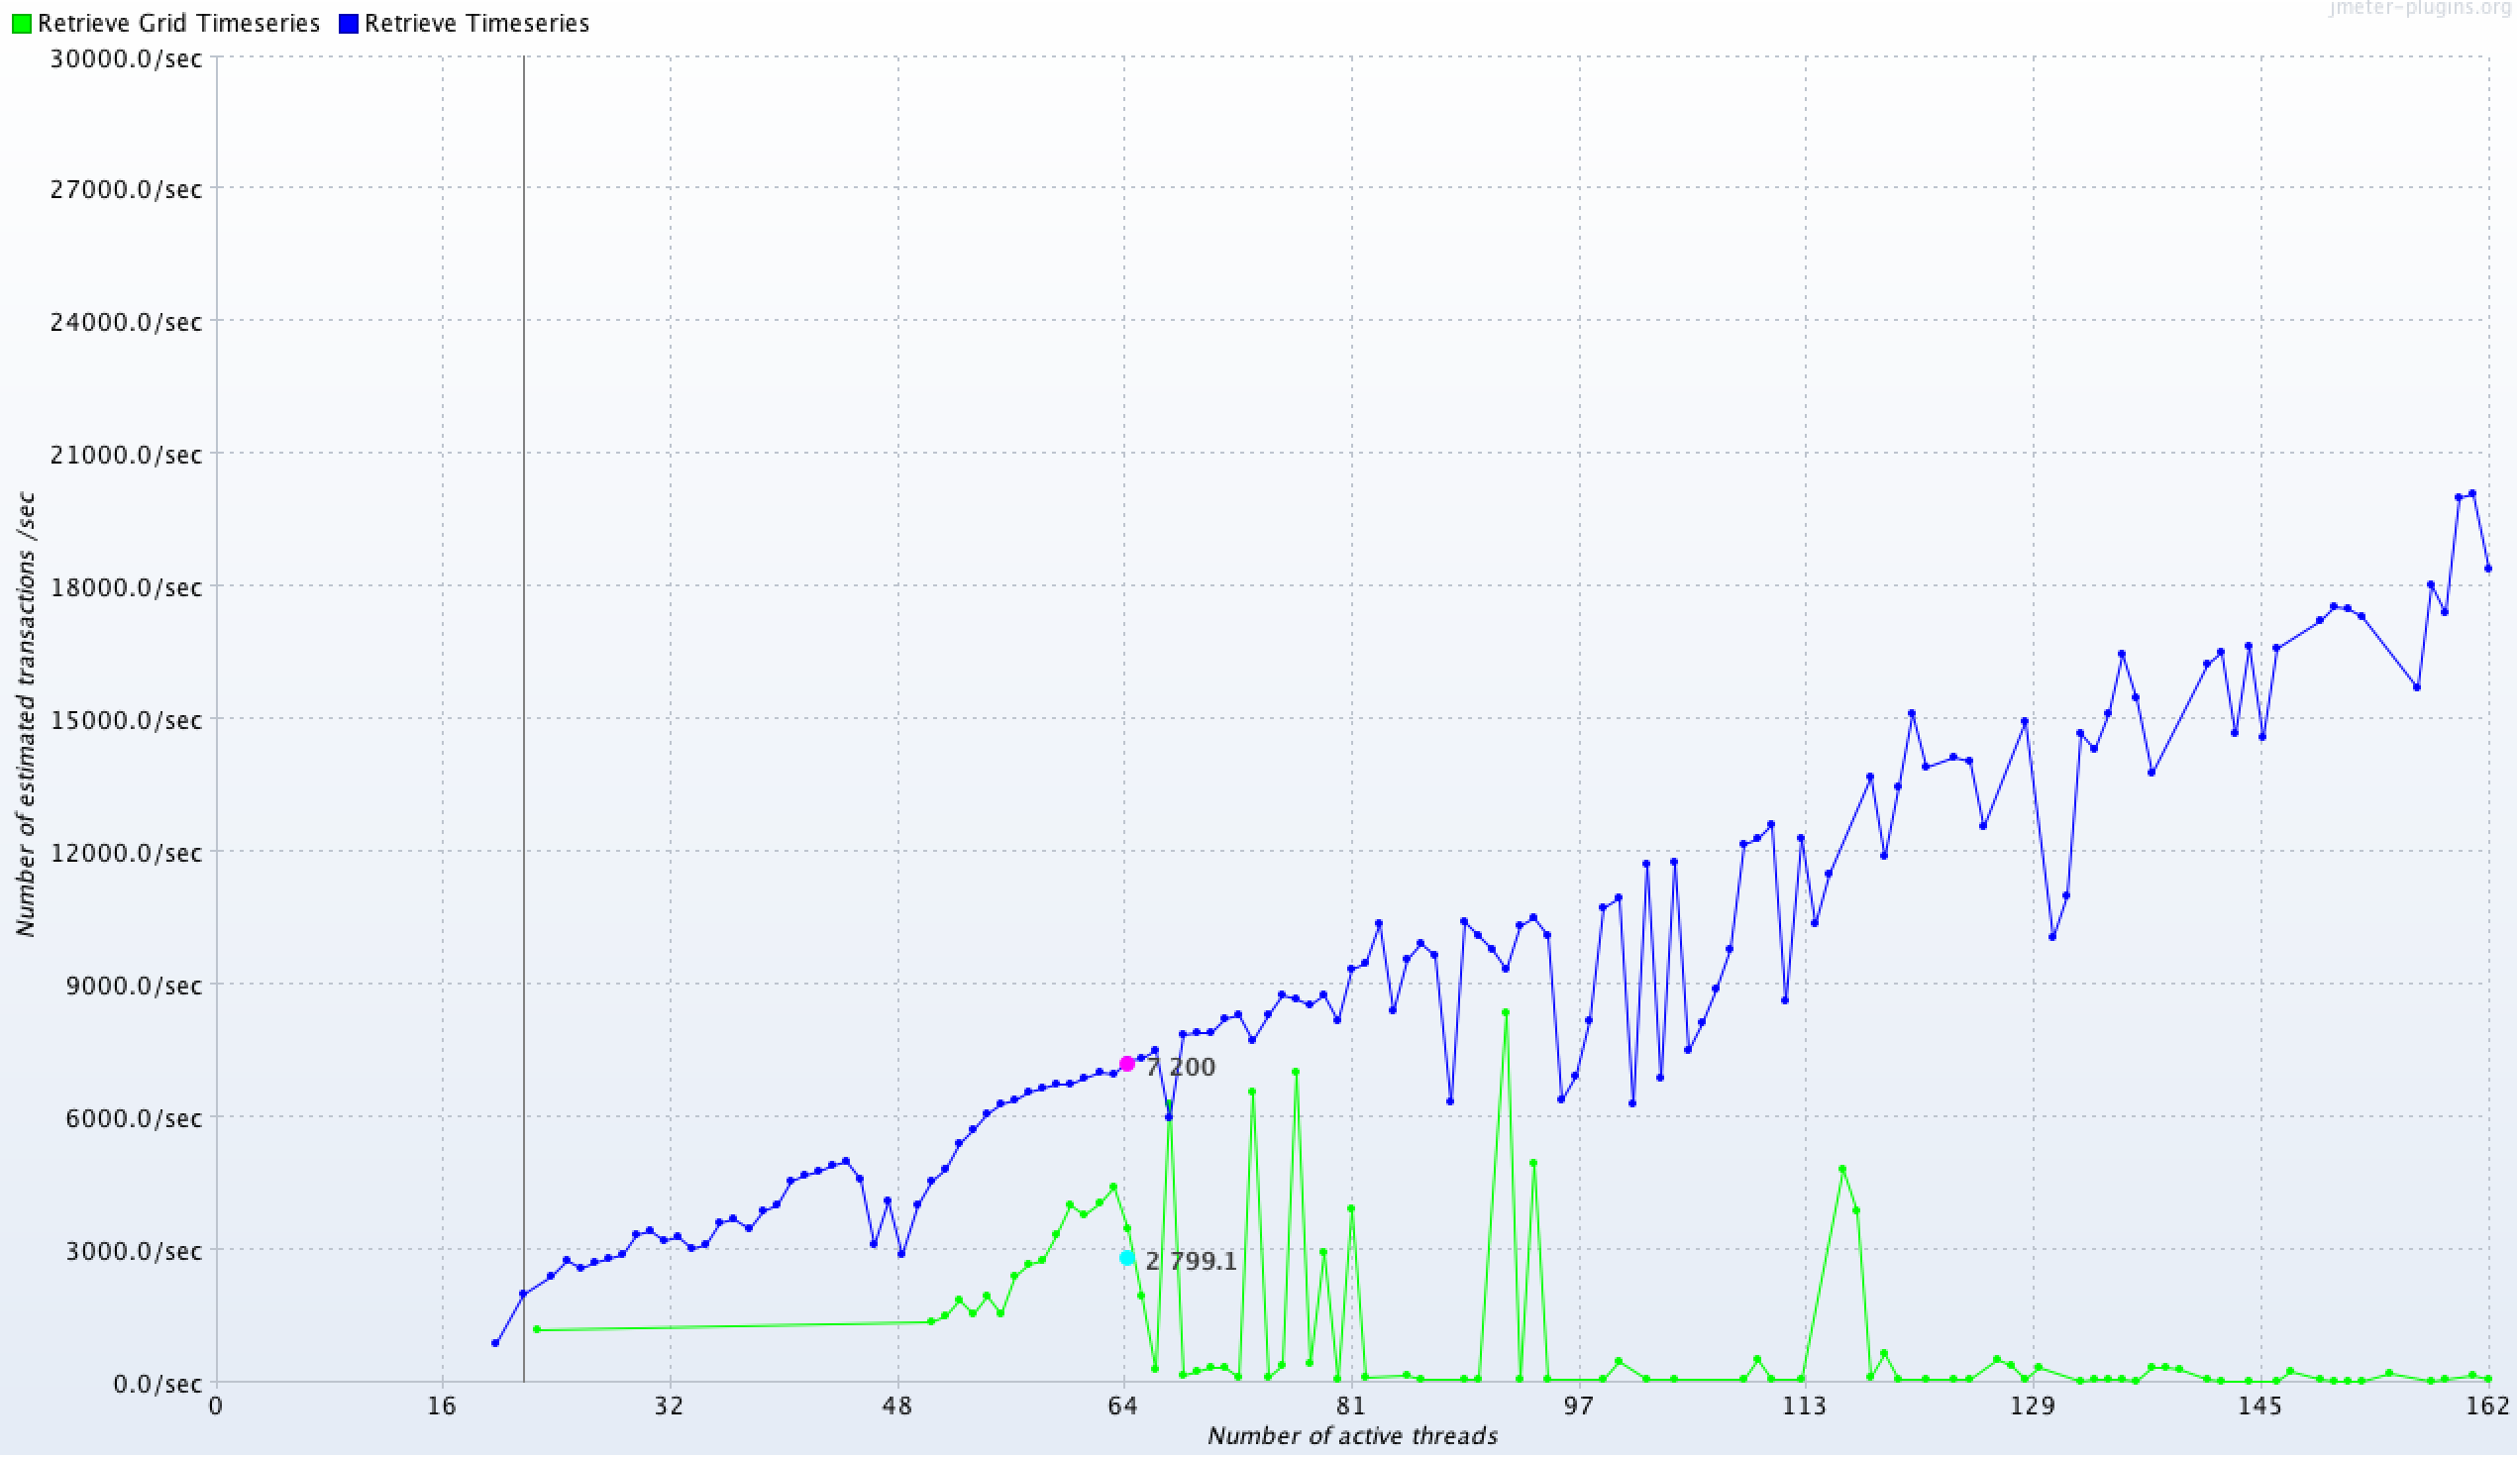
\includegraphics[width=0.8\textwidth]{results/obs/export/obs_export_15m_transaction_throughtput_vs_threads.png}
    \caption{Performance Export Test 15 minutes Interval - Transaction Throughput vs Threads}
    \label{fi:test_obs_export_15m_throughtput}
\end{figure}

\begin{figure}[htp]
    \centering
    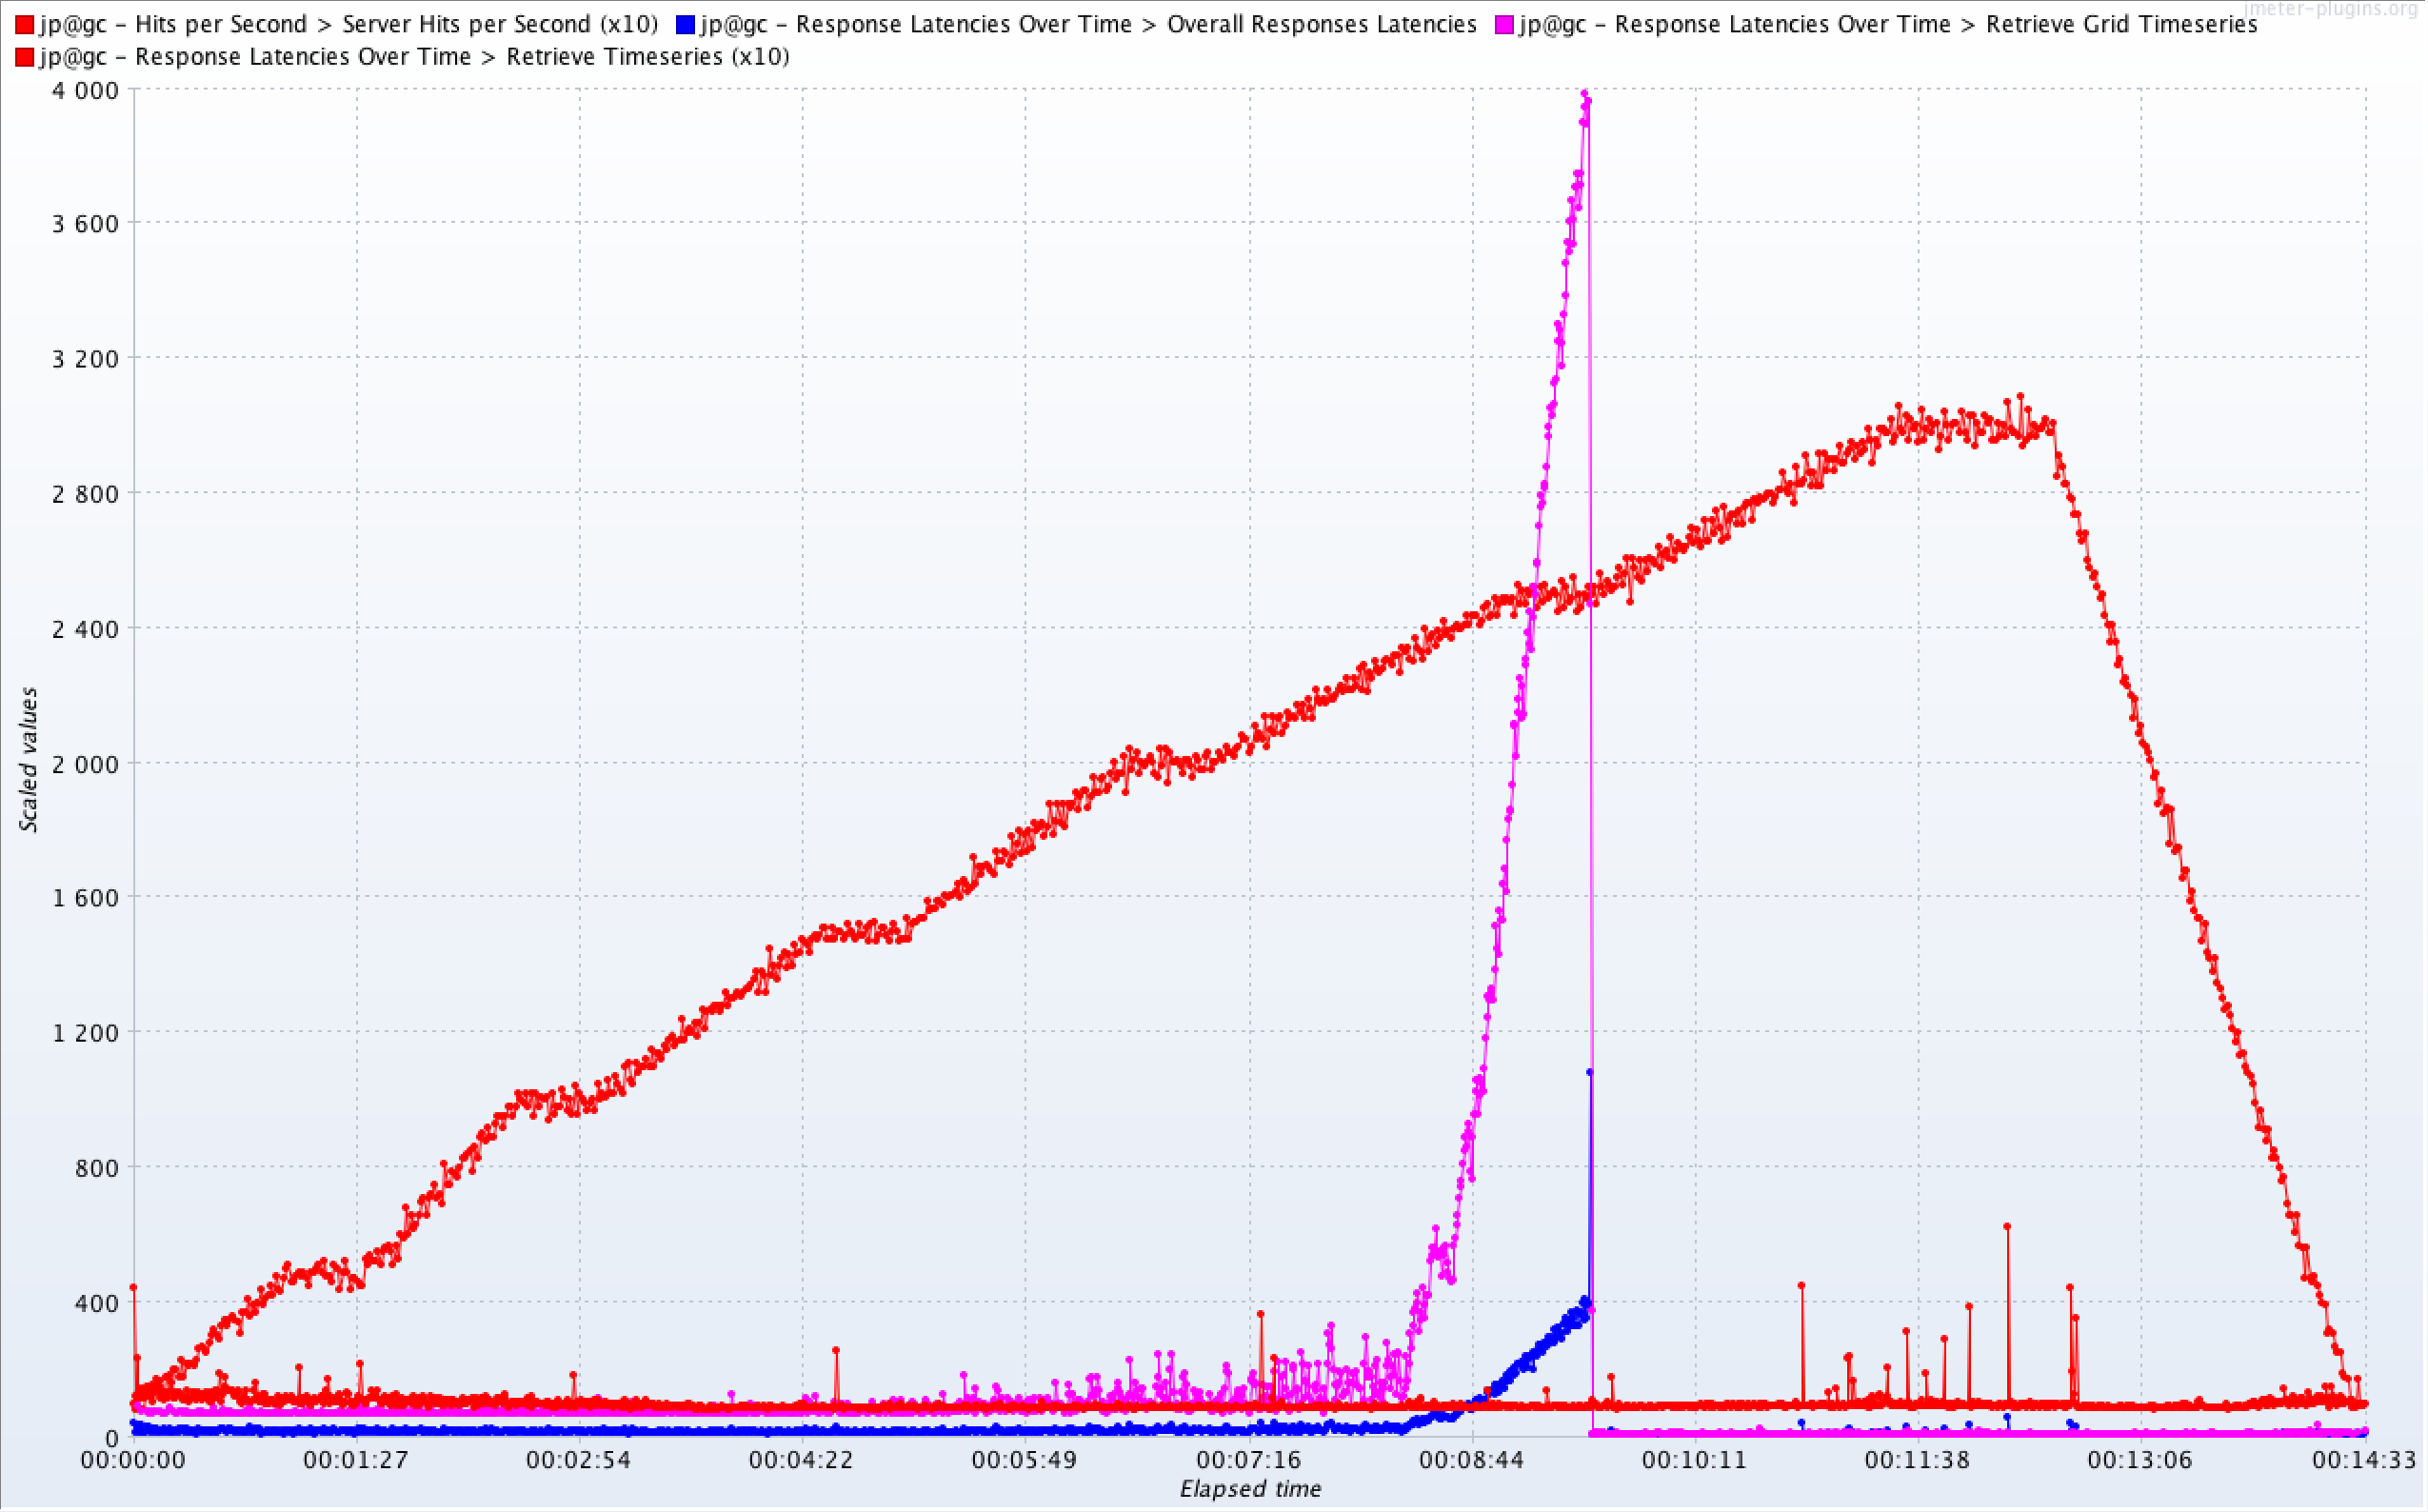
\includegraphics[width=0.8\textwidth]{results/obs/export/obs_export_15m_res_latencies_against_hits.png}
    \caption{Performance Export Test 15 minutes Interval - Latency against server hits}
    \label{fi:test_obs_export_15m_latency}
\end{figure}



\subsection{Extension module load test}



\subsection{Query module load test}

